\section{Numerical simulation algorithms} \label{chapter_numerical}
This section describes%{{{
the numerical methods used for preparation of this thesis. Major accent is put on the finite-difference time-domain method, since it was used for most simulations. Several important observations are discussed which are probably not found elsewhere. At its end, this chapter briefly mentions the plane-wave expansion method. 
%
%The finite-element method (FEM) appears to be the most widely used in computational electromagnetism today. It approximates the structure with a custom mesh of triangles or tetrahedra. The advantage consists in describing the structure smoothly with a relatively low number of elements of variable density; the disadwantage is in the fact that the computation of the tetrahedral mesh is significantly slower compared to straightforward arithmetics in FDTD. FEM is usually used as a frequency-domain solver, though time-domain computations are possible, too. The efficiency of the FEM mesh is superior to the FDTD/FDFD uniform grid particularly for structures with great differences between scale, that is, when important tiny structures are surrounded by large free space. This was however not the case of the structures studied in this thesis.
%
%Some methods are specific for partially periodic structures such as gratings, namely the \textit{rigorous coupled-wave analysis} (RCWA).
%% Boundary-element methods, Fourier modal method, 
%% discontinuous Galerkin method
%}}}
\subsection{Finite-difference time-domain method}
\paragraph{Algorithm desciption} %{{{
Finite-difference time-domain (FDTD) is one of the simplest methods for solving partial differential equations. The simulation volume is initialized as an array in the computer memory, each element of which corresponds to a \textit{voxel} in an orthogonal grid. When the FDTD method is applied to solve the Maxwell equations in three dimensions, six complex numbers per voxel describe the electric and magnetic vector fields, another static scalar arrays describe the permittivity and permeability of the structure and additional arrays may be used, corresponding to other physical quantities, such as material conductivity, polarizabilities and polarizations etc. 

The actual computation is realized in consecutive time steps as an explicit arithmetic operation on each voxel, taking into account only the field values in the neighboring voxels and in the previous time step \cite{taflove2005book} . This corresponds to iterating equations (\ref{eq_me3}), (\ref{eq_me4}) and (\ref{eq_ce}). % unclear - specify the field update routine exactly
Most of the computational time is thus occupied by a simple and unconditional loop repeatedly updating all voxels, which allows to fully employ the processor cache and facilitates multi-processor parallelisation. FDTD is applicable to (possibly non-linear) problems where either the temporal evolution of the fields is searched for, or for linear systems where a frequency-domain response function can be found by Fourier-transforming the time-domain response. 
% \begin{figure}[ht] \caption{A warning} \label{fg_parental} \centering 
% 	
\includegraphics[width=5cm]{img/Parental_Advisory_label.pdf}
% \end{figure}

The time-stepping routine needs the same computing power in empty vacuum as inside a complex structure. Grid-based methods such as FDTD are therefore the most efficient when a structure has relatively complex shape, but its smallest features are no more than two or three orders of magnitude smaller than the simulation size. In contrast, an accurate-enough simulation of a structure that has some few very fine features surrounded by big empty space would require an excessively high resolution, often resulting in the great majority of the voxels being inefficiently used in space where the high resolution is not needed. Other methods, % TODO discussed below
such as the finite-element method (FEM) or boundary-element method (BEM), would be preferable for such cases.

As widely used in the later chapters,  %% TODO illustrate it below!
simulations of a wave propagating in any periodic structure can make use of the periodic boundaries of the simulated volume, so that only one unit cell has to be computed to mimick an infinite lattice of these. The unit cells of periodic structures discussed in this thesis have their finest features not less than two orders of magnitude smaller than the unit cell size, and most of the simulations were aimed for obtaining a broadband spectrum, so FDTD was an optimal tool for this task.

%}}}
\paragraph{Spatial discretisation} %{{{ %% TODO add references
The discretisation of the grid and of the time stepping introduces an error that manifests itself in an imprecise description of the structure being simulated, known as \textit{staircasing} error. Another error arises in appreciable deviation of the light speed from the correct one at higher frequencies, the \textit{numerical dispersion} \cite{taflove2005book}.
\begin{figure}[ht] \caption{\textbf{(a)}, \textbf{(b)} Different two-dimensional grids are used for different polarizations of the fields. \textbf{(c)} The three-dimensional Yee grid. The electric field components are expressed in the centers of the cube edges which they are parallel to, whereas the magnetic components are expressed in the centers of the cube which they are perpendicular to. Note the electric and magnetic fields are completely equal in this scheme; the description in terms of edges and faces could be interchanged if the brown cube was taken as the elementary one.} \label{fg_fdtd_yee} \centering 
	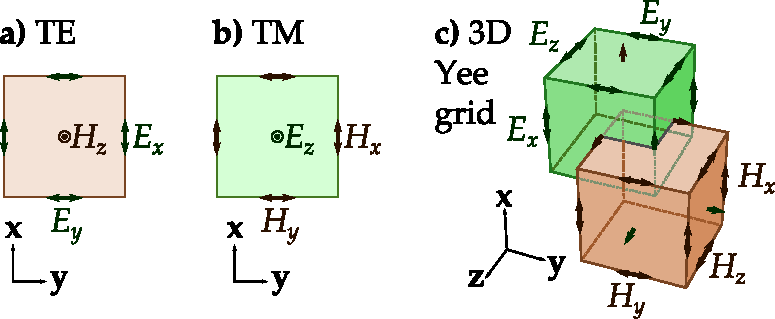
\includegraphics[width=12cm]{img/FDTD_Yee_grid_2d-3d.pdf}
\end{figure}

The error due to the numerical dispersion is in most FDTD implementations reduced from first to second order ($\propto \Delta x^{-2}$ with regards to the voxel size $\Delta x$) by using a \textit{staggered grid}, which, in three dimensions, is also known as Yee grid \cite{yee1966numerical}. All six field components are expressed in different points within the voxel, as is illustrated in Fig. \ref{fg_fdtd_yee}c.
Likewise, the update of electric and magnetic fields have to be interlaced also in time (as a so-called \textit{leapfrog} process). When accessing the field values at a given position and time, each field component has to be properly averaged between nearest points in the grid, and between nearest update times.  % NOTE FK: This can lead to errors especially at the boundaries with vacuum.

%}}}
\paragraph{Spatial discretisation} %{{{
By adequate averaging of permittivity on the boundaries of materials, this error can likewise be reduced to the quadratic order with regards to $\Delta x$. Various averaging approaches have been studied in the literature \cite{oskooi2010meep}. Arithmetic averaging of permittivity with a weight proportional to the voxel volume occupied by the material is perhaps the most intuitive one, but it often gives wrong results, and  sometimes it is even worse than no averaging at all \cite{farjadpour2006improving,deinega2007subpixel}. 

In case of a single planar interface between two different materials under general orientation, the arithmetic average of the permittivities $\varepsilon_r$ is correct only for the electric field component \textit{parallel} with the interface, whereas the component \textit{perpendicular} to the interface requires to apply this weighted averaging to the reciprocal value of permittivity, $\varepsilon_r^{-1}$, instead. Such an approach is extremely accurate for all interfaces with low curvature, but it requires the FDTD simulation to define the permittivity as a $3\times 3$ tensor array \cite{oskooi2009subpixel}. This is needed even in the case of using isotropic materials only. 

The situation gets even more complicated if the materials have dispersive permittivity, where also the weighting coefficients of both media need to be frequency-dependent, and another sophisticated approach has to be employed \cite{deinega2007subpixel,hamm2013dispersive}. Such a level of elaboration easily leads to computation requirements that may outweight the benefit of averaging, and accordingly no averaging was used for the simulations presented in this thesis. 

In general, the effect of discretization in FDTD simulations can be easily identified by comparing results from two simulations that only differ by the grid resolution. It is a good practice to verify that such an error is negligible whenever a new simulation is tested.
%}}}
\paragraph{Temporal discretisation} %{{{
While the spatial resolution $\Delta x$ can be relatively freely set depending on the accuracy expected by the user, the \textit{temporal resolution} $\Delta t$ is related to $\Delta x$ by rules that will be discussed below. Generally, if $\Delta t$ is set too high, the simulation will get numerically unstable, yielding unrealistic or even infinite values.  %  slowing down the computation and

In the literature, one often encounters that the \textit{Courant factor} $\cour$ is used instead of the description in terms of $\Delta t$,
\begin{equation} \cour = \frac{c \Delta t}{\Delta x}, \label{eq_courant}\end{equation}
In words, the Courant factor $\cour$ denotes what part of a FDTD cell the light can travel within one time step. 
The reason for introducing this quantity consists in the Maxwell equations [Eq. (\ref{eq_me1}-\ref{eq_me4})] being scale invariant, which holds also for the field update routine in FDTD when materials with frequency-independent permittivity are used. Therefore, when the resolution $\Delta x$ is changed, $\cour$ can be a well-chosen built-in constant and the time resolution given by Eq. (\ref{eq_courant}) ensures that the simulation does not go unstable.

FDTD obviously ceases to be scale-invariant whenever the properties of the materials depend on the frequency, which is needed for many realistic simulations. Then it appears more convenient to formally introduce yet another quantity, a \textit{critical frequency} $f_c$:
\begin{equation} f_c := \frac{1}{\pi \, \Delta t} \equiv \frac{c}{\pi\, \cour\, \Delta x} \label{eq_fc}\end{equation}
Note that this frequency is different %(i.e. $\pi$-times lower) 
than the frequency of time-stepping cycles is. From our observations, it is however the value of $f_c$, and its relation to the model of materials used, that are of key importance for assessing the numerical stability of simulation. %% TODO-FK: cite

%}}}
\paragraph{Definition of materials for the FDTD method} %{{{
\label{def_of_mat}

\begin{figure}[t] \caption{Plots of complex permittivity ${\epsrl}_o(\omega)$ of titanium dioxide (rutile), for an ordinary ray. The above plot has a linear vertical scale, while the bottom plot displays the same quantity using the scale that is $-\log(-\varepsilon_r)$ for $\varepsilon_r<-1$; linear for $-10<\varepsilon_r<10$ and $\log(\varepsilon_r)$ for $\varepsilon_r > 1$. The second approach better shows different orders of magnitude in the permittivity function.} \label{fg_tio2eps} \centering 
	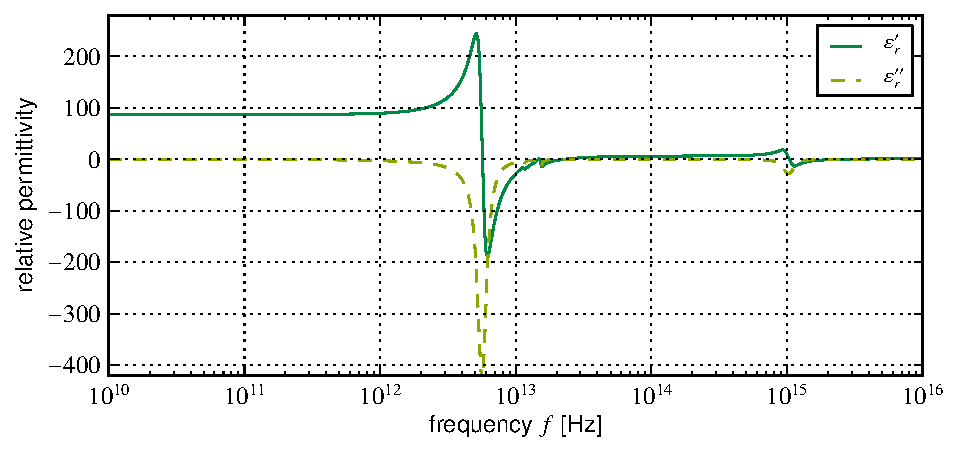
\includegraphics[width=14cm]{img/epsilon_TiO2_linear.pdf}
	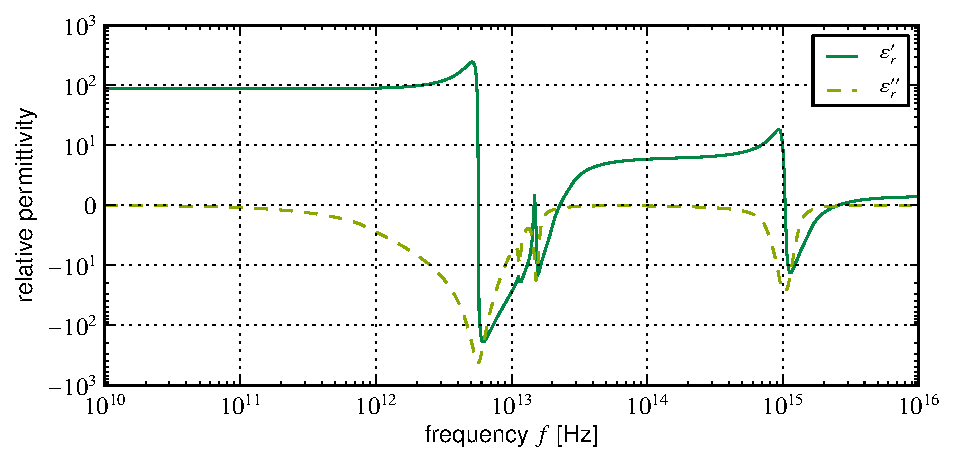
\includegraphics[width=14cm]{img/epsilon_TiO2_symlog.pdf}
\end{figure}

As described in Chapter \ref{chap_lorentzmedia}, Eqs. (\ref{eq_lorentz_eps}, \ref{eq_lorentz_mu}), the local response of usual media to an electromagnetic wave can be well approximated by a set of Lorentz oscillators, each of which is defined by three positive real numbers: its resonance angular frequency $\omega_{0}$, damping rate $\gamma$ and oscillator strength $F$. % todo cite 

%It is not possible to directly supply the permittivity as an arbitrary function of frequency from fundamental reasons. 
%We thus return to the local Drude-Lorentz theory, with a due emphasis on the definition of materials in FDTD.
% we focus on this topic because in literature, either general theory is discussed, or just single working model  is used. We try to develop reliable rules for employing the FDTD to simulate realistic structures under as general circumstances as possible.
FDTD, being a time-domain method, uses %% TODO-FK why?
a computationally efficient description of the media in a similar  form, with the difference that the nondispersive part of relative permittivity $\varepsilon_{r\infty}$ can be chosen as a real number. 
\begin{equation} \epsrl(\omega) = \varepsilon_{r\infty} + \sum_{m=1}^M \frac{F_m}{\omega_{0m}^2 - \omega^2 + \ii\omega\gamma_m} \label{eq_lorentz_eps_fdtd} \end{equation}
An illustration of a complex permittivity spectrum for titanium dioxide in its rutile allotrope is shown in Fig. \ref{fg_tio2eps}. As its crystal is birefringent, only one permittivity component, denoted as the \textit{ordinary}, from the tensor in Eq. (\ref{eq_epstensor}) was selected. 


% TODO add a spectrum + table for SiO2?
%			or exp(-i omega t)					-> fourier transform has to be conjugated (??)


%A rough list of the most important phenomena follows. 
%\begin{table}[ht]   \caption{}  \label{tb_phenomena} \centering 
%\begin{tabular}{lcr}
 %\toprule
%Frequency $\omega_0/(2\pi)$         & Contribution $\Delta\varepsilon_r$ & Physical phenomenon	\\
 %\hline
%---									& 0--10000 &	& Rotation of polar molecules	\\
%1 THz -- 30 THz						& & Vibration of atomic lattice	\\
%200 THz - 1000 THz					& &	\\
 %\bottomrule
 %\end{tabular} \end{table}
%\begin{enumerate}
 %\item{In the low frequency and microwave range (up to 1 THz), rotation and reorganisation of polar molecules plays the major role in the medium polarizability. } 
 %\item{Depending on the hardness and density of the medium, the lattice vibrates at frequencies between 1 and 30 THz.} 
 %\item{The frequencies corresponding to  electron motions of solids are in near-infrared, optical or ultraviolet ranges (roughly 200-1000 THz).}
 %\end{enumerate}
%If the medium is conductive, 

%}}}
\paragraph{Conditions of stability in FDTD}%{{{
%it was noted above that too high frequency of oscillators may introduce instability. 
%An important parameter is the critical frequency of the simulation, $f_c$ defined as 
% \begin{equation} f_c = \frac{c}{\pi \, C \, \Delta x},\label{eq_}\end{equation}
% where the \textit{Courant factor} $C$ is usually set to $C:=0.5$ and $c \approx 2.998 \cdot 10^8$ m/s is the speed of light. The voxel size thus determines the critical frequency; in a simulation typical for this thesis, $\Delta x := 2$ $\upmu$m and the critical frequency $f_c \approx 95$ THz lies in the mid-infrared. For simulations in visible range with $\Delta x := 50$ nm, and $f_c \approx 3800$ THz, that is, in the regime of hard UV radiation.

%The critical frequency may be viewed as the upper limit where an FDTD simulation gives plausible data. 

The author observed that $f_c$ determines the constraints for the simulation stability simultaneously in two ways:
\begin{enumerate}
 \item{The resonance frequencies must be lower than the critical frequency,  %% TODO get a proof, or some citation, or cite MEEP sources where S.G.Johnson wrote a routine about this
\begin{equation} \frac{\omega_{0m}}{2\pi} < f_c, \text{ for all oscillators, } % \forall m \in \{1,2 \ldots M\}, \label{eq_fdtd_stability}
\end{equation}
independent of what the strength $F_m$ or damping rate $\gamma_m$ of the oscillator is. 
%This relates to the above note about expressing all high-frequency oscillators in the form of the high-frequency (static) permittivity. . 
} 
 \item{For all frequencies higher than the critical frequency $f_c$, the real part of the permittivity, as given by Eq. (\ref{eq_lorentz_eps_fdtd}), must exceed a minimum value given by the Courant factor $\cour$,
\begin{equation} \varepsilon_r'(2\pi\,f) > 3 \cour^{2} \equiv 3 \left( \frac{c \Delta t}{\Delta x} \right)^{2} \text{ for } \forall f \geq f_c. \label{eq_fdtd_stability_realp}\end{equation}  } % TODO verify whether the limit is eps>0 or e.g. eps>0.5 or whatever 
A geometrical interpretation of this rule is that an instability is introduced when any wave with a frequency above $f_c$ can travel more than $1/\sqrt{3}$ of one FDTD cell size within one time step. 
Note that in a nonmagnetic medium, the traveled distance is $$\frac{c\Delta t}{\sqrt{\varepsilon_r'}}.$$
\end{enumerate}
Both rules were observed to hold in media with $\murl = 1$ only; in media with magnetic response they would be probably more complex.
The FDTD simulation will become unstable if one of these rules is broken. The error from the instability initially arises from an inevitable numerical noise at the boundary of the problematic material and grows exponentially. It can be identified as a pixel-wise checkerboard pattern on the field snapshot. Later, the field visualisation usually returns black images as the numerical infinity is reached within several tens of FDTD steps. 

\paragraph{Choice of the Courant factor}%{{{
Provided that a part of the simulation volume is empty vacuum ($\varepsilon_r'=1$), Eq. (\ref{eq_fdtd_stability_realp}) clearly determines the \textit{maximum value of Courant factor} 
$$\cour_{max} = 3^{-1/2}\approx0.577.$$
In practice, a slightly more conservative choice is made that provides a safe margin for the numerical imprecision: 
\begin{equation} \cour:= 0.500 \quad \rightarrow \quad \varepsilon_r'(2\pi\,f)> 0.75, \quad \forall f \geq f_c. \label{eq_courant_choice}\end{equation}
For any material with a problematic high-frequency permittivity, $\varepsilon_r'(2\pi\,f_c) \in (0, 1)$, some low value of $\cour$ can be found that makes the simulation stable against the latter rule. Simultaneously, the critical frequency shifts up, so potential problems with the first rule may be alleviated, too. This is done, however, at the price of scaling up the number of required FDTD steps, so usually a reasonable change of the material definition is made instead of reducing $\cour$.
%% TODO note that the same would apply to permeability mu, but it usually does not have problematic oscillator parameters

%%% TODO 
%%% This is related to the \textit{Courant criterion} \cite{taflove2005book} that states for a nondispersive medium of permittivity $\varepsilon_r$ that 
%%% $$\Delta t = \cour\,\frac{\Delta x}{c}  <  \frac{\sqrt{\varepsilon_r}}{\sqrt{3}}   \frac{\Delta x}{c}$$, as $\cour < n_{min}/\sqrt{\text{dim}}$ % TODO
%%% i.e.
%%% $$c \Delta t / n_{min} < \Delta x / \sqrt{\text{dim}} $$
%%% which can be reformulated that   %TODO TODO

%  /* Return true if the discretized Lorentzian ODE is intrinsically unstable,
%     i.e. if it corresponds to a filter with a pole z~outside the unit circle.
%     Note that the pole satisfies the quadratic equation:
%  			(z + 1/z - 2)/dt^2 + g*(z - 1/z)/(2*dt) + w^2 = 0
%     where w = 2*pi*omega_0 and g = 2*pi*gamma.   It is just a little
%     algebra from this to get the condition for a root with |z| > 1. */
%  static bool lorentzian_unstable(double omega_0, double gamma, double dt) {
%    double w = 2*pi*omega_0, g = 2*pi*gamma;
%    double g2 = g*dt/2, w2 = (w*dt)*(w*dt);
%    double b = (1 - w2/2) / (1 + g2), c = (1 - g2) / (1 + g2);
%    return b*b > c && 2*b*b - c + 2*fabs(b)*sqrt(b*b - c) > 1;
%  }
%}}}


%The first rule of $\omega_0/2\pi < f_c$ was observed to be very strict
%}}}
\paragraph{Practical aspects of material definition} %{{{
In all realistic media, the frequencies of different oscillators span over many orders of magnitude, and an accurate medium model would need to determine excessively big number of oscillators. Not all oscillators should be accounted for in a given FDTD simulation, however. 

\begin{figure}[t] \caption{Permittivity plot for titanium dioxide, similar to Fig. \ref{fg_tio2eps}. 
%Compared to the exact model of permittivity (green line), the model with reduced number of Lorentz oscillators was plotted (black line). 
The region forbidden by the stability rules is yellow shaded (above $f_c = 95$ THz and below $\varepsilon_r < 0.75$). The exact model for TiO$_{2}$ (green line, from Ref. \cite{dominec2014_meep_metamaterials}) would be definitely unstable due to violating both stability conditions. The numerically stable model for the frequency range of interest up to ca. 10 THz (black line) has all high-frequency oscillators substituted by an increased value of $\varepsilon_{r\infty}$. Solid and dashed lines denote the real and imaginary parts, respectively. } \label{fg_tio2eps_stripped} \centering 
	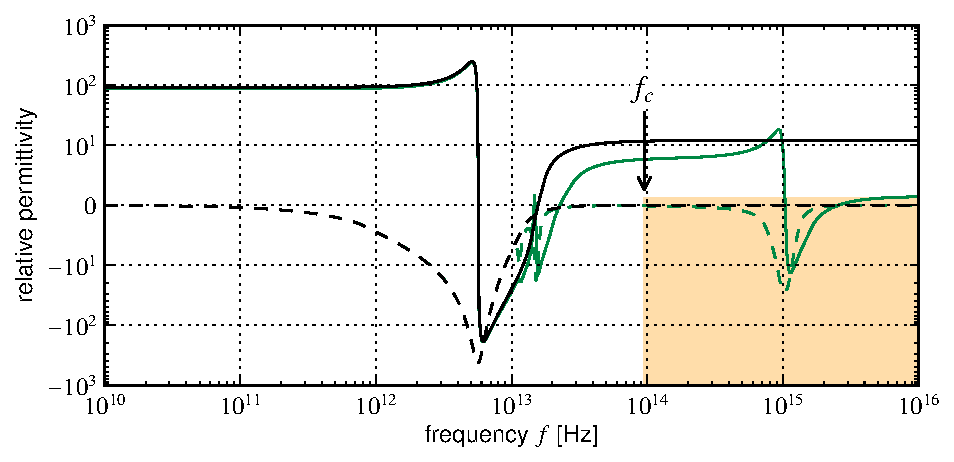
\includegraphics[width=14cm]{img/epsilon_TiO2stripped_symlog.pdf}
\end{figure}

First of all, high-frequency oscillators would make the simulation unstable.
Aside from this, adding overly many oscillators is also inefficient, because each oscillator defined increases the computing difficulty in FDTD. 
It is therefore advisable to keep the oscillator number to an acceptable necessary minimum, and to describe the material within some frequency range of interest (FRoI) % TODO  define range of interest
only:
\begin{enumerate}
 \item{
%Often the first step in processing FDTD results lies in converting them to frequency domain via Fourier transform. 
The upper bound of the FRoI is limited by the numerical stability as stated above. Mostly, a more strict limit is imposed by the spatial resolution of the simulation: in a high-permittivity material, too high frequencies correspond to wavelengths similar to the voxel size (or even smaller than it), leading to a significant inaccuracy. 

Each oscillator far above the frequency of interest shall be expressed only as a constant added to the nondispersive part of permittivity $\varepsilon_{r\infty}$. The contribution of an $m-$th oscillator is given by Eq. (\ref{eq_delta_eps}) as 
$$(\Delta \varepsilon_r)_m = \frac{F_m}{\omega_{0m}^2}.$$ 
If some of the high-frequency oscillators introduces significant dispersion or losses in the FRoI, it it should not be eliminated this way. This usually concerns the oscillator that is the closest above FRoI, and it usually can be kept without causing instability.
} 
 \item{
Very low frequencies, corresponding to wavelengths much greater than the whole simulation volume, are theoretically accessible with a long-enough FDTD simulation, but it would not be practical to extend the FRoI close to the zero frequency. If needed, the low-frequency phenomena can often be computed more efficiently in a separate simulation with a lower resolution or even with different numerical methods.

The oscillators at too low frequencies can therefore be omitted without any change to the behaviour within the FRoI. One important exception is the low-frequency oscillator that stands for the Drude term and defines the conductive behaviour, as described below.
} 
 \end{enumerate}
%}}}
\paragraph{Drude model for conductive media} \label{chap_fdtd_drude}  %{{{
The Drude model assumes a zero resonance frequency, i.e., the relative permittivity in the form
\begin{equation} \epsr(\omega) = 1 + \frac{\omega_p^{2}}{0 - \omega^{2} + \ii\gamma\omega} = 1 - \frac{\omega_p^{2}}{\omega^{2} - \ii\gamma\omega}, \label{eq_drude_eps}\end{equation}
where $\omega_p$ and $\gamma$ are two independent parameters that describe the metal: 
\begin{itemize}
 \item{$\omega_p$ is the \textit{plasma frequency}, at which the real part of permittivity crosses zero. The physical consequence is that for $\omega > \omega_p$ the medium allows the transverse electromagnetic wave to propagate through. 
%The angular frequency of $\omega_p$, the longitudinal (electric) waves oscillate. 
%The quasiparticle associated with the oscillation of the charge in bulk conductive medium, a \textit{plasmon}, has given the name to $\omega_p$. % TODO add a relation to the chapter on "dispersion in local media"
 } 
 \item{$\gamma$ can be understood as the \textit{rate of exponential decay} of the medium response to an impulse, similar as in the Lorentz model. The Drude model was conceived in the early 20th century, with the simplified hypothesis that electrons would be freely propagating particles that undergo 
	% mutual elastic %% +FK?
collisions 
	with the atoms %% -FD?
at an average frequency $\gamma$. Upon the colision, their 
	%speed would either drop to zero, or (equivalently) %% -FD?
	velocity vector % + FK
would be randomized. 
%Although the mechanism of resistivity is more complicated than this,  -FD
The Drude model often provides a very good approximation of the metallic-like response.
The parameter $\gamma$ is commonly denoted as the \textit{scattering frequency}.} 
 \end{itemize}
%Both have the dimension of $\mathrm{rad\; s^{-1}}$. 
The Drude model can thus be considered a specific case of a Lorentz oscillator with $\omega_0 = 0$, and oscillator strength given by $F = \omega_p^2$. 
Obviously, using Eq. (\ref{eq_delta_eps}) to compute the contribution of the Drude term to the real part of permittivity would give infinite values, as static electric field can displace unlimited amount of charge in a conductor.

If $\gamma$ is nonzero, the permittivity is a complex function and it can be separated into its real and imaginary part $\varepsilon_r = \varepsilon_r'+\ii\varepsilon_r''$ by expanding the fraction in (\ref{eq_drude_eps}) by complex conjugate of its denominator
\begin{equation} \varepsilon_r = 1 - \omega_p^{2} \cdot \frac{\omega^{2} + \ii \gamma \omega}{\omega^{4} + \gamma^{2} \omega^{2}} = 
		\underbrace{\left(1 - \frac{\omega_p^2}{\omega^2+\gamma^2}\right) }_{\text{real part } \varepsilon_r'}
+ \ii	\underbrace{\left(\frac{-\omega_p^2\gamma}{\omega^3 + \gamma^2\omega}\right) }_{\text{imaginary part } \varepsilon_r''}.
\label{eq_drude_eps_loss}\end{equation}
%The real part $\varepsilon_r'$ indicates capacitive or reactive behaviour of the metal. The imaginary part $\varepsilon_r''$ describes losses which may arise either from 
% \underbrace{ }_{\text{}}
The low- and high-frequency limits of permittivity given by the Drude model are:
\begin{equation} \lim_{\omega \to 0} \varepsilon_r' = 1-\frac{\omega_p^2}{\gamma^2}, \quad \quad  
				 \lim_{\omega \to 0} (\varepsilon_r'' \cdot \omega) = -\frac{\omega_p^2}{\gamma},\label{eq_drude_limlow}\end{equation}
\begin{equation} \lim_{\omega \to +\infty} \varepsilon_r' = 1, \quad \quad  
				 \lim_{\omega \to +\infty} (\varepsilon_r'' \cdot \omega^3) = -\omega_p^2 \gamma. \label{eq_drude_limup}\end{equation}
We can see that in the low-frequency limit, the imaginary part of permittivity diverges (while its real part has a finite value). In the high-frequency limit, the metal permittivity approaches that of vacuum, i.e. $1+0\ii$.
%}}}
\paragraph{Low- and high-frequency limits of conductivity in the Drude model}%{{{
The notion of \textit{conductivity} is widely used to describe metals and doped semiconductors, i.e. media where the response to the electric field is characteristic by the motion of free charge carriers. 
Generally, both permittivity $\varepsilon_r(\omega)$ and conductivity $\sigma(\omega)$ are complex functions of the angular frequency $\omega$. As long as the approximation of a negligible spatial dispersion is used, each of them is fully determined by the other function. % maybe even if spatial dispersion is nonzero -> check this?
For clarity, we avoid using the conductivity in the rest of the thesis except this chapter.

The relation between $\varepsilon_r(\omega)$ and $\sigma(\omega)$
 can be derived by realizing that the current in a material is always caused by movement of charges with a density $j$ and average velocity $\mathbf{v}(t)$. The conduction and polarisation currents are not distinguished here, as their density is given as $j \mathbf{v}(t)$ in both cases. When current is excited by a harmonic electric field $E(t) = \mathrm{e}^{\ii\omega t}$: %TODO FIXME explain j.n, use i omega t instead of -i omega t, check again...
\begin{equation} j \mathbf{v}(t) = \sigma(\omega) E(t) = \sigma(\omega) \mathrm{e}^{\ii\omega t}, \quad\text{ (conduction approach -- Ohm law)} \label{eq_rho_n1}\end{equation}
\begin{equation} j \mathbf{v}(t) = \varepsilon_0 \varepsilon_r(\omega) \frac{\partial E(t)}{\partial t} = \ii \omega \varepsilon_0 \varepsilon_r(\omega) \mathrm{e}^{\ii\omega t} . \quad\text{ (displacement current approach)} \label{eq_rho_n2}\end{equation}
Both above equations describe the same quantity, so
\begin{equation} \sigma(\omega) = \ii \omega \varepsilon_0 \varepsilon_r(\omega), \quad  \text{and} \quad  \varepsilon_r(\omega)  = \frac{\sigma(\omega)}{\ii \omega \varepsilon_0}. \label{eq_drude_sigma}\end{equation}
Thus, a dielectric medium with a real constant permittivity has \textit{imaginary} conductivity, the magnitude of which grows with frequency (cf. the admittance of a capacitor). A conductor with a real constant conductivity has complex permittivity, whose imaginary part diverges in the low-frequency limit. 
% NOTE: eps_r = eps_r' + i eps_r'',   
% sigma = sigma' + i sigma'' == i omega eps0 eps_r == i omega eps0 eps_r' - omega eps0 eps_r''
% therefore a material can be described also using real epsilon = eps_r', and real conductivity sigma' = -omega eps0 eps_r''

\begin{figure}[t] \caption{Permittivity and conductivity plot for gold; the yellow region, forbidden by the stability rules, is the same as in Fig. \ref{fg_tio2eps_stripped}. The exact model of gold \cite{rakic1998optical} 
(red) is compared to the lossy Drude model with Lorentz oscillators substituted by $\varepsilon_r$ (blue), and for illustration, also to the lossless Drude model with scattering frequency set to zero (grey). Obviously, none of these models is numerically stable if $f_c = 95$ THz.
\\The bottom plot shows the conductivity of these three models as given by Eq. (\ref{eq_drude_sigma}).}
\label{fg_Au_models} \centering 
	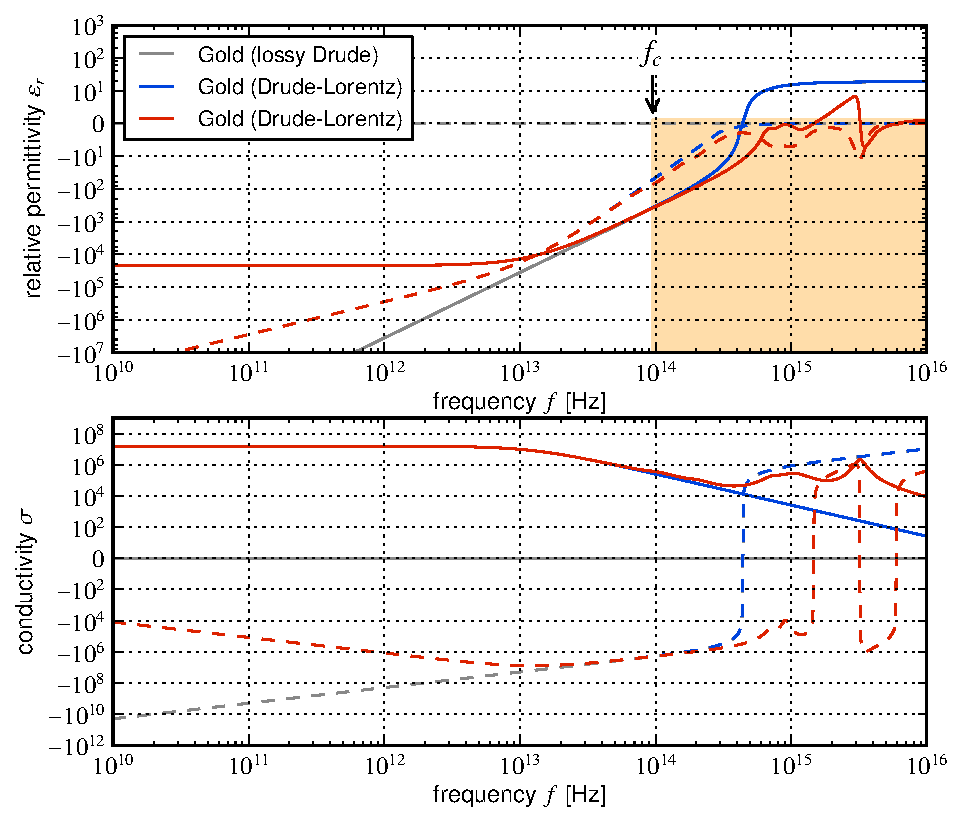
\includegraphics[width=14cm]{img/epsilon_Au_models_llgrey.pdf} % Scattering freq of gold = 12.8 THz
\end{figure}


Using the above relation (\ref{eq_drude_sigma}) to convert the metal permittivity $\varepsilon_r(\omega)$ into conductivity $\sigma(\omega)$, and substituting the Drude-model permittivity (\ref{eq_drude_eps_loss}), we obtain
\begin{equation} \sigma(\omega) = \ii \omega \varepsilon_0 \varepsilon_r(\omega)= \ii\omega \varepsilon_0 \varepsilon_r'(\omega)  -  \omega \varepsilon_0 \varepsilon_r''(\omega) = 
	\ii \underbrace{\varepsilon_0 \left(\omega - \frac{\omega_p^2\omega}{\omega^2+\gamma^2}\right)}_{\text{imaginary part } \sigma''}  + 
		\underbrace{\varepsilon_0\frac{\omega_p^2\gamma}{\omega^2+\gamma^2}}_{\text{real part } \sigma'}. \label{eq_drude_sigmaeps1}\end{equation}
We may now express the low- and high-frequency limits also for conductivity:
\begin{equation} \sigma_{LF} := \lim_{\omega \to 0} \sigma' = \frac{\omega_p^2\varepsilon_0}{\gamma}, \quad \quad  
				 \lim_{\omega \to 0} (\sigma'' / \omega) = \varepsilon_0 - \frac{\omega_p^2 \varepsilon_0}{\gamma^2} , \label{eq_drude_sigmalimlow}\end{equation}
\begin{equation} \lim_{\omega \to +\infty} (\sigma' \cdot \omega^2) = \varepsilon_0\omega_p^2\gamma, \quad \quad  
				 \lim_{\omega \to +\infty} (\sigma'' / \omega) = \varepsilon_0. \label{eq_drude_sigma_limup}\end{equation}
Let us note again that in the literature that uses the negative phase convention $e^{-\ii \omega t}$, the resulting $\varepsilon_r(\omega)$ and $\sigma(\omega)$ are complex conjugated to the results above. 
%}}}
\paragraph{Defining resistive metals for stable low-resolution simulations} %{{{
Simulations in the optical range are relatively safe in terms of numerical stability. From Eq. (\ref{eq_fc}) it follows that the resolution of $\Delta x = 50$ nm, suitable for the NIR/visible spectrum, yields a critical frequency of $f_c = 3.82\cdot 10^{15}$ Hz ($\lambda = c/f_c \approx 78$ nm), which is far above the plasma frequency of metals or other conductors. Accordingly, no changes to the Drude model are usually needed to be made, although the simulation may run faster if one or more Lorentz terms outside FRoI can be omitted.
%If high precision of the metal model is needed, one is also free to add one or more Lorentz oscillators in the optical/UV range to refine the shape of permittivity.
 
Realistic simulations of metals at lower resolutions however require taking measures to ensure stability, as the critical frequency $f_c$ is reduced below the plasma frequency of most metals when $\Delta x \gtrsim 200$ nm. % TODO check this
A trivial approach is to drastically reduce the Courant factor $\cour$ so that $f_c$ remains above plasma frequency. Although this should reliably avoid the instability, it would be so at the expense of scaling the computational time. As a general rule, lower resolution is typically chosen for larger structures, where also all investigated processes accordingly happen on a longer timescale.
%Drude model is known to introduce negative permittivity up to optical range, so 
%Assuming the critical frequency is far below the optical range, the Lorentz oscillators can be certainly neglected. Nonetheless, negative permittivity above critical frequency still introduces instability, which has to be resolved. 

For simulations with lower resolution, it is much more efficient to replace the exact Drude model with its approximation that maintains the same low-frequency limit of conductivity $\sigma_{LF}$, but has positive permittivity around the critical frequency and above it. 
This formally inverts the relations that describe the material:
\begin{itemize}
\item{
For \textit{high-resolution simulations}, $\omega_p$ and $\gamma$ are given as experimental properties of the metal, which determine the lower limit $\sigma_{LF} = \omega_p^2\varepsilon_0\gamma^{-1}$ and the nondispersive part of permittivity $\varepsilon_{r\infty} = 1$ is fixed to that of vacuum. 
} 
\item{
For \textit{low-resolution simulations}, the situation is the opposite: $\sigma_{LF}$ is given as an experimental property, $\gamma < 2\pi f_c$ is given by the critical frequency, % TODO describe why so
whereas $\varepsilon_{r\infty}$ and $\omega_p$ are to be determined from the previous two input parameters.
} 
\end{itemize}

%%% TODO
%%% 	% In this section we develop the strategy to determine the correct combinations of  $\gamma < 2\pi f_c$, $\varepsilon_{r\infty}$ and $\omega_p$.
%%% 	% The value of $\gamma$ is also limited to be lower than $2\pi f_c$, so its value is fixed to be as close to $2\pi f_c$ as possible. % TODO ...is it? verify and add to the rules for stability written above
%%% 	 The values of the plasma frequency $\omega_p$ as well as the  $\varepsilon_{r\infty}$ remain to be freely manipulated.
%%% 
%%%     $$ \gamma = 2\pi f_c \cdot gammafactor $$
%%%     % test when unstable -> reduce self.gamma by 100 -> test again -> finally write automatic selection of value
%%% 
%%%     % Knowing the scattering frequency gamma, the virtual plasma frequency is now determined by lfconductivity
%%%     $$ \omega_p = \sqrt{\frac{\gamma \sigma_{LF}}{\varepsilon_0}} $$
%%% 
%%%     % The following step is required for FDTD stability: 
%%%     % Add such an high-frequency-epsilon value that shifts the permittivity to be positive at f_c
%%%     % If self.eps>1, the frequency where permittivity goes positive will generally be less than f_p
%%%     $$\varepsilon_{r\infty} = (\omega_p/(2\pi f_c))^2 \text{ or 1 if it would be lower} $$

%}}}
%\paragraph{Conductive media in FDTD} %{{{
%The resonance frequency $\omega_0$ is inversely proportional to the square root of the restoring force in the harmonic oscillator. A conductive medium is characteristic by having part of the charges that do not experience any restoring force, so they can be modelled by an oscillator with a resonance frequency approaching zero: $\omega_0 \rightarrow 0$; in practice any value lower than the inverse of simulation time gives expected results.
%When $\omega_0$ is reduced to small values, the oscillator epsilon difference $\Sigma = \Delta \varepsilon_r$ has to be upscaled accordingly to keep the plasma frequency constant.
%When $\omega_0$ is reduced to small values, the oscillator strength $F$ shall be kept constant?
%}}}
\paragraph{Debye media in FDTD} \label{fdtd_debye} %{{{
The Lorentz model can be employed also to define overdamped oscillators, corresponding to the processes where  $\gamma \gg \omega_0$, i.e. the inertia is negligible.
A typical example is the  reorientation of polar molecules in liquids or solids. 

It can be shown that for $\gamma \gg \omega_0$, the peak in $\varepsilon_r''(\omega)$ lies approximately on the frequency $\omega_p^{2}/\gamma$. The spectral width of such a peak is proportional to its central frequency. 
% TODO figure illustrating this

\begin{table}[ht]   \caption{Comparison of Lorentzian types and corresponding physical phenomena}  \label{tb_lorentzians} \centering 
\begin{tabular}{cc|cc}
 \toprule
\textbf{Charges are}	& \textbf{Charge inertia is}				& \textbf{Phenomenon}				& \textbf{Example}		 \\
 \hline
Bound		& Significant				& Lorentz oscillator					& \shortstack{optical phonons, \\electronic levels,\\ molecular vibration \\or rotation in gases}	\\
 \hline
Bound		& Negligible				& Debye relaxation						& \shortstack{molecular rotation \\in solids or liquids} \\
 \hline
Free	    & Significant				& \shortstack{Reactive\\(plasmonic) medium}			& \shortstack{colisionless plasma, \\metals (from mid-infrared\\to optical range)} \\
 \hline
Free	    & Negligible				& Resistive medium						& \shortstack{doped semiconductors,\\\newline metals (in far-infrared\\ range and below)} \\
 \bottomrule
 \end{tabular} \end{table}
%}}}
% TODO? \paragraph{Selection of FDTD implementations} %{{{
% note about the meep peculiarity of notation: 'omega'=omega0/2pi , 'gamma'=gamma/2pi, 'sigma'=Deltaeps = F/omega0^2
%MEEP, OpenEMS, B-Calm, gSvit, EMTL, ..
%}}}

\subsection{Finite-difference frequency-domain method} % TODO
\paragraph{Principle}  %{{{
When the procedure for one time-step in FDTD is defined, it can serve as the linear operator $\mathcal L$ in the generic formulation of the eigenfunction problem:
$$\mathcal{L} \psi = e^{\ii \omega t} \psi,$$
where the function $\psi$ represents either of the electric or magnetic fields. 
%The particular form for the linear operator $\mathcal{L}$ is  as has already been developed for the proof of the Bloch theorem in Eq. (\ref{eq_eigen_e}).
% TODO maybe not! The Hamiltonian might be SQUARE of the "Maxwellian"!

Both time- and frequency-domain simulations used for this thesis use complex numbers to represent all field components.
Whole frequency-domain problem thus can be expressed as a simultaneous optimization of the $\E(\rr), \HH(\rr)$ fields, so that one time-step of FDTD is as similar as possible to the phase rotation of the functions. The angle of the phase rotation is given by the user-defined angular frequency $\omega$. For the optimization to be as efficient as possible, the \textit{stabilized biconjugate gradient} algorithm \cite{oskooi2010meep} is used. More information on the frequency-domain solver is on the project's website \cite{ab-initio}. 

The modes obtained by frequency-domain simulation can be output with arbitrary phase; sometimes the real part of either electric or magnetic field can be nearly zero. In such a case, the imaginary part thereof always gives sufficient amplitude to be plotted accurately.

%}}}
\paragraph{Comparison to the time-domain computation} %{{{
To verify their reliability, the results of the frequency domain simulation with frequency scanned were compared against the results from the time-domain simulation. 

The advantage of the frequency-domain (FDFD) method over the time-domain (FDTD) is greater efficiency for obtaining the field shape at a single frequency, where the computational time of the time-domain methods grows proportionally with the desired spectral resolution. Having both algorithms packed in one library enables extremely easy switching between them. 

While the spectra of all material properties in FDTD have to conform to the Kramers-Kronig relations, in FDFD the permittivity and conductivity of each medium can be chosen without any limitations.
A frequency scan of multiple FDFD simulations can thus be more efficient for simulation of superconductors or materials with too many resonances.  

It was observed by the author that the FDFD solver in the MEEP program often fails to converge when plasmonic effects at the optical frequencies. In such cases, one has to replace it the FDTD algorithm with a narrow frequency source.

%}}}

\subsection{Plane-wave expansion method} % TODO
\paragraph{Description} %{{{
Another algorithm used in this thesis is the \textit{plane-wave expansion method} (PWEM). Whereas FDTD and FDFD are very general algorithms that can be applied for different choices of simulation setups and for virtually any structure, PWEM is specialised for periodic structures only. 

Each PWEM computation is always performed for one given value of the wavevector $\KK$. PWEM resolves one or more frequencies which lie on the dispersion curve of the Bloch wave $\omega(\KK)$. For each of them, it can also output the shape of the mode function $\mathbf{u_{e,m}}(\rr)$. The algorithm is described in detail, e.g., in Ref. \cite[pp. 24-28]{pazoutova2011dp}.

As a convenient implementation of PWEM, we used the freely available program \textit{MPB} \cite{johnson2001mpb}, provided as open-source project by the same group \cite{ab-initio} as MEEP. Graphical presentation of the results was prepared using a custom script published online \cite{dominec2015_mpb}.

%}}}
\paragraph{Comparison to FDTD and FDFD} %{{{
The electric and magnetic field shapes at the edges of each photonic band are important for understanding the physics of periodic structures. Note that the fields inside a photonic band do not usually share the periodicity with the lattice, which makes them harder to interpret. Finding the band edges is an intrinsic feature of PWEM, whereas the same task is only approximate in FDTD and requires previous search for the band edge frequencies. 

Scaling of the computational time with the resolution may present a disadvantage compared to FDTD/FDFD, since in a simple implementation it scales with second power of the resolution for one-dimensional problems, fourth power in 2-D problems and ninth power for 3-D problems. Application of more sophisticated algebra of sparse matrices can however partially remedy this.

Perhaps the greatest limitation of the MPB program is that it can not cope with negative permittivity values. Its applicability is thus restricted to fully dielectric structures only.	

%}}}

%\subsection{Summary of numerical methods used} %{{{
%This section describes several fundamentally different numerical methods for electromagnetic simulations. 
%\begin{enumerate}
%\item{Finite-difference time-domain (FDTD) is a time-marching method that describes the structure on an uniform grid, allowing to compute very general electromagnetic problems. Usually a short-time, broadband pulse excitation is used, which allows to resolve a broad spectrum at once by Fourier transform. In the following chapter, two fundamentally different setups for FDTD are described that provide similar information on the metamaterial.} 
%\item{The finite-difference frequency-domain (FDFD) method uses the same discretisation as FDTD, but instead of time-marching and Fourier transforming the result, it searches for the field eigenmode at one given frequency by means of numerical optimisation. It is useful e.g. for mode analysis in complicated structures.} 
%\item{The plane-wave expansion method (PWEM) reformulates the problem of a wave propagating in a periodic structure by means of linear algebra. At a given wave vector, it allows to find eigenmodes and eigenfrequencies in the structure. This can be in turn employed to efficiently retrieve the dispersion curves.} 
%\item{The transfer-matrix method (TMM) also allows to find dispersion curves and field distribution. Although it can be extended to two or three dimensions, its one-dimensional implementation is most popular. Thanks to its simplicity, it can even give an analytical insight into the behaviour of planar structures.} 
%\end{enumerate}
%}}}

\section{Simulation setups for metamaterial homogenization} 
The general electromagnetic algorithms,%{{{
such as FDTD, FDFD or FEM, can be employed to find the electromagnetic field behaviour in a wide variety of problems. These algorithms, however, tell nothing about the effective parameters of a metamaterial, unless they are employed in a particular simulation setup. 

This section describes two different setups we have implemented, the retrieval of scattering parameters and the current-driven homogenisation. Other setups can be found in the literature, too, and are briefly mentioned at the end of this section.
% TODO theoretically shown in works [12,13,14,15] and experimentally confirmed in [16] this technique is not applicable when the sample material experiences the resonance
%		[12] C.R. Simovski, S.A. Tretyakov, Phys. Rev. B 75 (2007)195111
%		[13] C.R. Simovski, Metamaterials 1 (2007)62
%		[14] C.R. Simovski, Metamaterials 2 (2008)169
%		[15] C.R. Simovski, Optics and Spectroscopy 107 (2008)726
%		[16] Kh.Chalapat, K.Sarvala, J.Li, G.S.Paraoanu, IEEE Transactions on Microwave Theory and Techniques 57 (2009)2257
%}}}
\subsection{Scattering parameters retrieval} \label{chapter_sparam}
\paragraph{Principle} %{{{
The scattering parameter retrieval, also known as the \textit{s-parameter}, \textit{distributed impedance} or \textit{Nicolson-Ross-Weir} (NRW) method \cite{nicolson1970measurement, weir1974automatic}, has been used since 1970s to experimentally retrieve the index of refraction $N$ and wave impedance $Z$ of a homogeneous material sample.

The first step to its derivation is that by means of the Fresnel-Airy formulas \cite[p. 329]{born1999book},
one can easily compute the transmission $t(f)$ and reflection $r(f)$ spectra from a slab of any material, provided its thickness $d$, index of refraction $N$ and wave impedance $Z$ are known.  If $r,t$ are known instead, the Fresnel-Airy formulas can be inverted to yield $N$ and $Z$ of the material the slab consists of. The actual computation is thus denoted also as \textit{Fresnel inversion}.

Mathematically, this can always be done. When the homogeneous sample is replaced by an inhomogeneous structure, such as a layer of a metamaterial unit cells, this method still yields some \textit{effective} parameters, $\Neff(f)$ and $\Zeff(f)$, the relevance of which is discussed later. 

As a great advantage of this approach, there is no requirement to inspect the fields inside the tested structure, as the retrieval is based only on the amplitude and phase of the  $r(f)$ and $t(f)$ outside the material. It has become a popular way to retrieve the effective metamaterial parameters thanks to its ease to realize both experimentally and numerically, with FDTD or other algorithms \cite{terao2011},

The most often mentioned downside of this method is that its solutions have infinitely many branches, and it is necessary to establish which one should be chosen, and why. In this section we describe that this can, in fact, be solved by a relatively simple extension of the algorithm, and in the Results chapter it is shown that there are nontrivial rules for the choice of the branch.

Aside from yielding multiple branches, the physical interpretation of the data can get even more intricate when effective parameters are to be assigned to an inhomogeneous slab of a metamaterial. Due attention has to be paid to minimize the intrinsic imprecision of this method, as well as to establish the limits of its applicability. 
%}}}
\paragraph{Simulation setup} %{{{
\begin{figure}[ht] \centering \caption{The simulation setup for the scattering parameter method. All simulation elements are described in the text.
% TODO REWRITE, and add the X-Y-Z arrows to the figure}
} 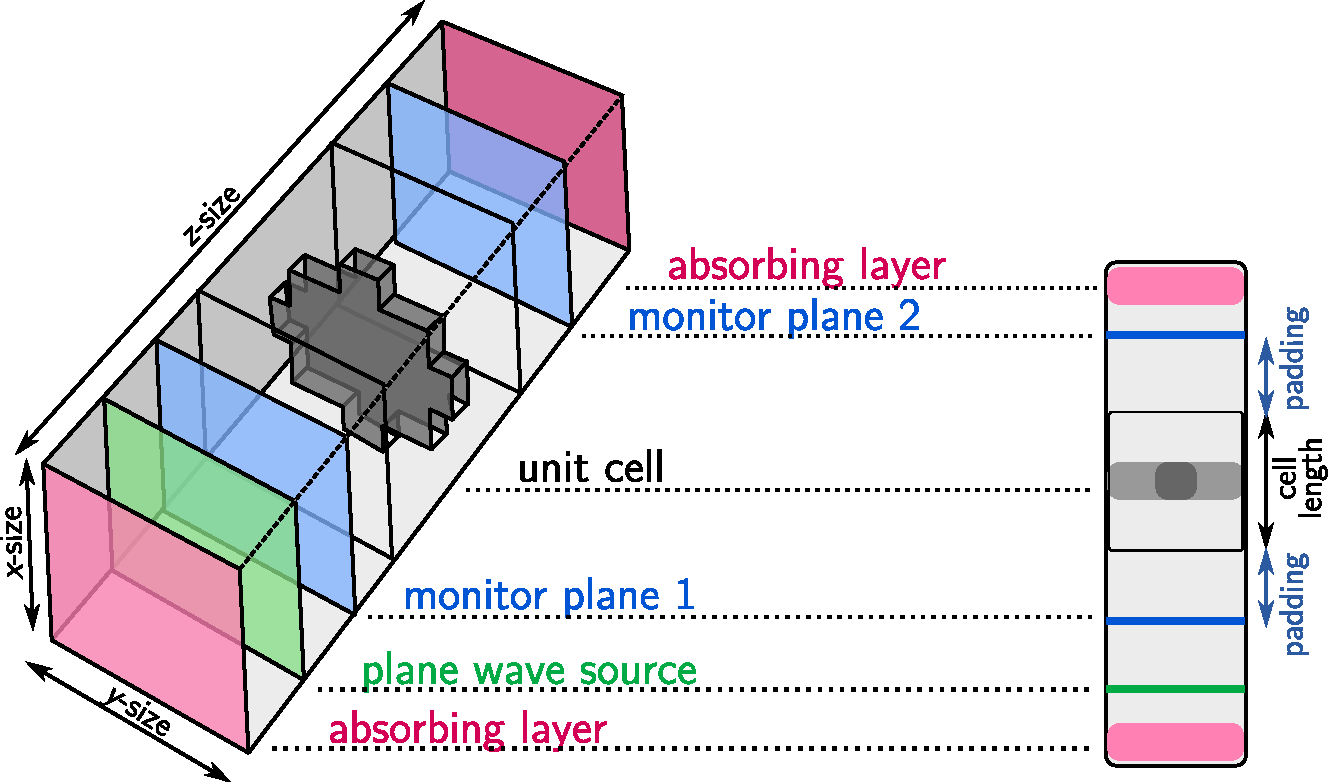
\includegraphics[width=.8\textwidth]{img/meep_geometry.pdf}  \label{fg_fdtd_sparam} \end{figure} %% 
The setup for the scattering parameter methon is depicted in Fig. \ref{fg_fdtd_sparam}. The wave is emitted from the source plane (green rectangle) with a direction parallel to the $z$-axis. The temporal shape of the wave was not critical for the simulation; a very short pulse, with a spectrum spanning from the GHz range to ca. 5 THz was used. 

The periodic boundary conditions were set on the $x$- and $y$-axes, so that effectively an infinite metamaterial slab was simulated. On both faces perpendicular to the $z$ axis we added regions denoted as \textit{perfectly matched layers} \cite{oskooi2011distinguishing} to absorb all radiation (pink blocks). The implementation used is based on gradually introducing imaginary part into the unit cell dimensions to prevent reflections under arbitrary incidence angle, polarisation or frequency of the wave.
The average electric and magnetic fields in each of the monitor planes (blue rectangles) are recorded  in each simulation step.  

Passing through the first monitor plane, the wave enters the volume of the unit cell (delimited by empty rectangles) and interacts with the structure. A part of its energy is reflected back, a part passes through and the rest may be dissipated if the structure is lossy. The fields that pass through the structure are recorded by the second monitor plane. After the energy stored in the structure drops to a small enough level, the FDTD simulation terminates and the recorded fields are processed to obtain the complex-valued reflection $r(f)$ and transmission $t(f)$ as functions of frequency $f$. % Before this procedure is described, a modification important for the accuracy of this setup is discussed below.
% todo convert frequency f to omega? Why not?

%\begin{figure}[ht] \caption{An example result of a FDTD simulation (visualised using the \textit{Paraview} program). A dielectric sphere, shown in grey, was placed in a less usual, but equivalent position, across the periodic boundaries. The electric field amplitude was shown in one quarter of the simulation volume, with a clear enhancement near the dielectric surface (pink-red). % todo{replace this with a better one}
%}  \centering 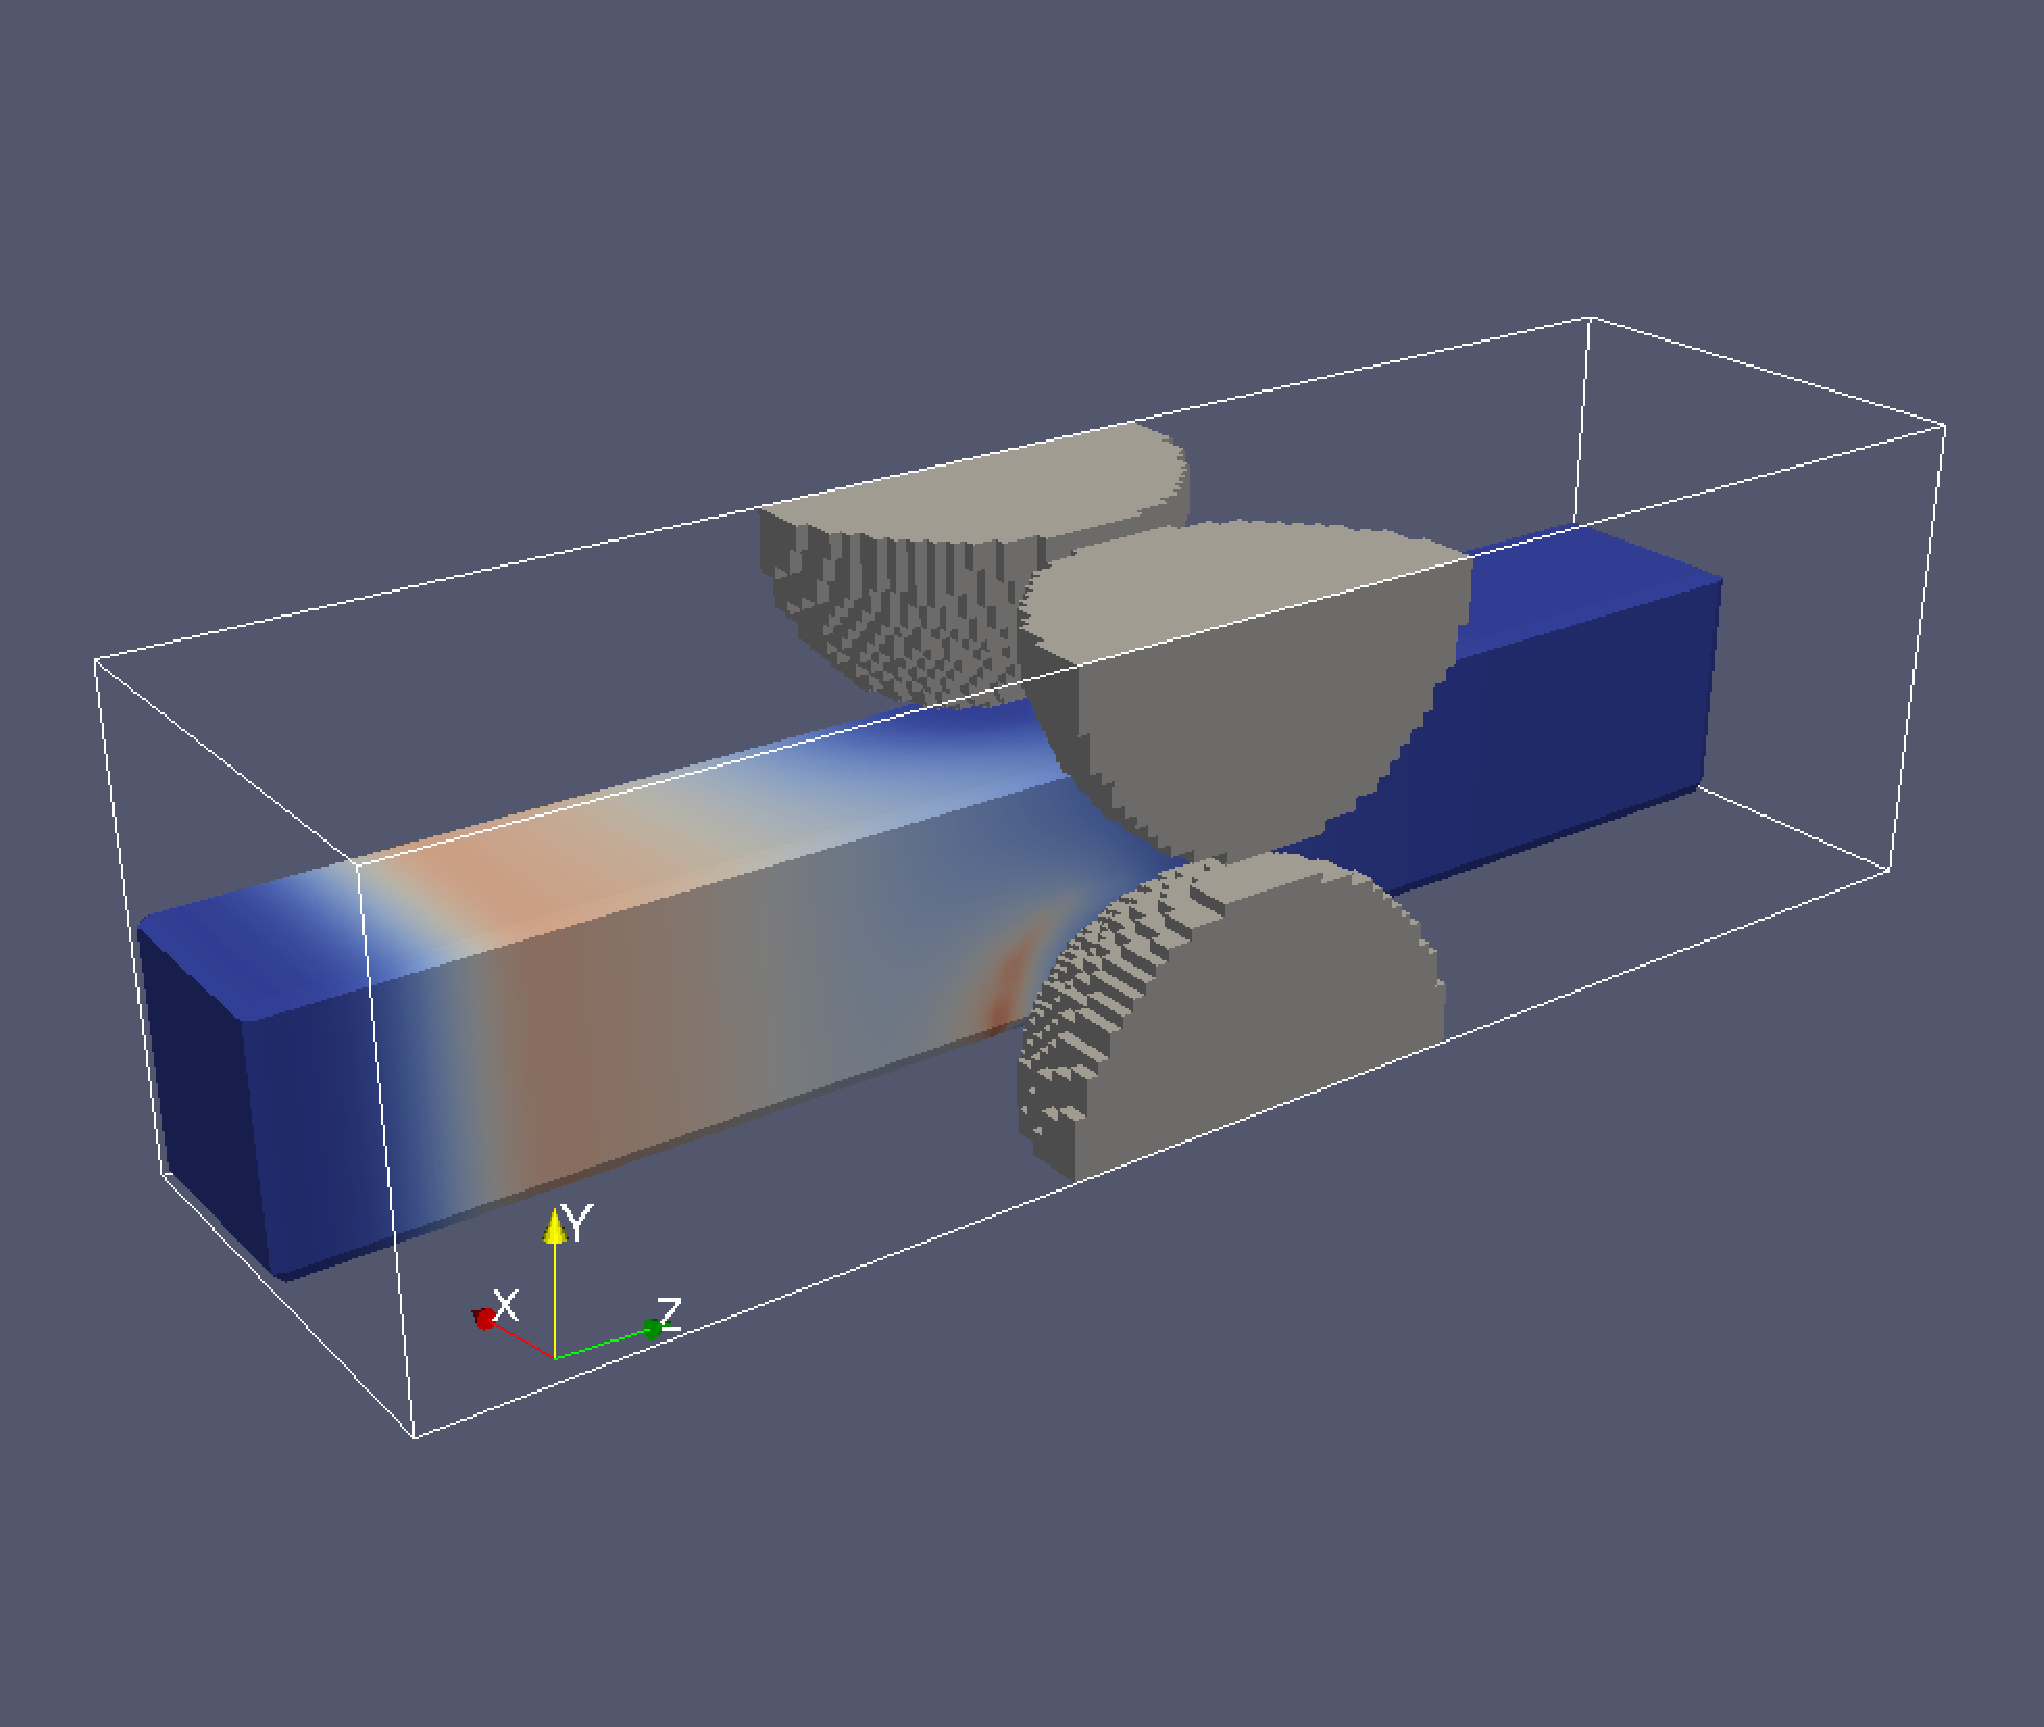
\includegraphics[width=10cm]{img/sim_screen.pdf} \label{fg_fdtdscreen} \end{figure} 
%}}}
\paragraph{Avoiding the near-field response in monitor planes} %{{{
\label{par_nearfield}
%% Hynek's trick
With the obvious exception of an effectively one-dimensional structure of layers perpendicular to the wave propagation, all other structures will change also the orientation of the electric and magnetic fields. Such a perturbation of the field will be localized around the structure, and exponentially decaying with the distance in the form of an \textit{evanescent wave}.

An evanescent wave does not transport energy out of the structure into free space. However, some energy is stored in it, which can be transmitted to another structure if it approaches the zone of the evanescent wave. Aside of this, even if no energy is transferred by this means, the electromagnetic behaviour of a structure is always slightly influenced by its surroundings, which manifests itself most often as resonances shifting up or down in frequency.

The impact of the evanescent wave partially reaching the unit cell boundaries in the s-parameters method is twofold:
\begin{enumerate}
 \item{First, computing a single layer of a metamaterial unit cells, with free space in front and behind it, obviously more or less changes its behaviour compared to the periodic lattice. 

This issue is inherent to the simulation setup, but its impact can be assessed by simulating more than one unit cell, since the retrieved values will change slightly with the number of layers being simulated: a single-cell simulation suffers the most from the absence of adjacent layers, whereas in a two-cell simulation the effect should be halved. Simulations of three (or more) cells suffer from a different behaviour of the cells at the surface and inside, which possibly broadens the resonance frequency and can yield confusing results unsuitable to the retrieval method.
 } 
 \item{Second, the monitor planes can not distinguish between the evanescent or radiated electromagnetic field, but only the radiated waves are relevant for the s-parameter computations. At very low frequencies or at frequencies close to resonances, it was observed that the near field can significantly distort the retrieved parameters.

This can be resolved by shifting both monitor planes away from the metamaterial cell by a distance denoted as \textit{padding}. As the evanescent field decays exponentially, padding of less than half of the unit cell size is sufficient to suppress all artifacts due to near-field components. In contrast, propagating waves only gain an additional phase offset that can be easily compensated after the simulation. } 
 \end{enumerate}
To the knowledge of the author, such a shift of monitor planes has not been employed in any related paper. It efficiently resolves the issue, and it does so at an acceptable expense of moderately extending the simulation volume. % (todo? figure here a-b-c of different padding near a dielectric rod)

%}}}
\paragraph{Scattering-parameter retrieval procedure} %{{{
The averaged electric and magnetic fields recorded at the first monitor plane will be denoted as $E_{x}^{(1)}(t), H_{y}^{(1)}(t)$. Likewise, those at the second monitor plane will be denoted as $E_{x}^{(2)}(t), H_{y}^{(2)}(t)$. The amplitudes of typical time records are shown and commented in a logarithmic scale in Fig. \ref{fg_sparam_timedomain}.  
\begin{figure}[ht] \centering \caption{Time-domain records of the fields in the s-parameter-based retrieval method; absolute values of the complex recorded fields at the first $E_{x}^{(1)}(t), H_{y}^{(1)}(t)$ and second $E_{x}^{(2)}(t), H_{y}^{(2)}(t)$ monitor plane.\\
The excitation pulse ca. 2 ps long excited in the structure two distinct resonances that both decayed exponentially in time with different decay rate, as is outlined by thin line segments. About 35 ps after the source was switched off, the stronger resonance reduces its intensity below that of the higher quality resonance, which can be clearly seen as a change of the decaying amplitude slope. The simulation time  was $t_{sim} =$ 150 ps. \\
After 80 \% of the time record length, the field is multiplied by the smooth envelope function described by Eq. (\ref{eq_envelope}).} 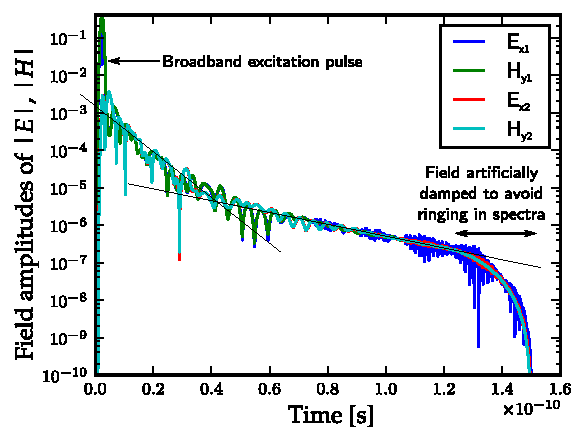
\includegraphics[width=.7\textwidth]{img/sim_timedomain_debug.pdf} \label{fg_sparam_timedomain} \end{figure}

The spectral resolution is determined by the length of the time record. The higher quality of resonance, the sharper its spectral features. %is equivalent to coarse sampling on the frequency axis, which can not fully resolve the shape of the resonance. 
From the \textit{Fourier-Plancherel theorem} %% TODO ref
it follows that the part of the electromagnetic energy which was coupled to the structure, but was not radiated back until the end of the time record, will be also missing in the spectra in the frequency domain. When the time record is too short and significantly truncates a resonance ring-down, characteristic artifacts in the spectra occur which are very detrimental to further visual and numerical evaluation. 

\label{convolringing}
Using the convolution theorem (see Sect. \ref{subsection_local_resp}), it can be deduced that clipping the recorded fields by a rectangular window in time domain introduces artifacts equivalent to a convolution with the sinc function in the frequency domain. Multiplication of the records with a smooth window function, known also as \textit{apodization}, does not improve spectral resolution, but it suppresses the visually distracting artifacts. Therefore, all four time records were multiplied by the envelope function $g(t)$ before further processing:
\begin{equation} 
\begin{split}
	g(t) 	& = 1 \text{ for } t < 0.8 t_{sim} \\
	g(t)    & = \frac{1 + \cos\left(\pi \frac{t/t_{sim}-0.8}{1-0.8}\right)}{2}  \text{ for } t > 0.8 t_{sim},
\end{split}
\label{eq_envelope}\end{equation}
which ensured that after 80 \% of the overall simulation time $t_{sim}$ the field starts dropping smoothly to zero, similar to the \textit{Hann window} function often used in digital signal processing. 

By means of the Fourier transform, the fields were converted to the frequency domain. This operation is simply denoted as $E_{x}^{(1)}(t) \rightarrow E_{x}^{(1)}(f)$, and so on. 
\begin{figure}[ht] \caption{An illustration of how the electric field $\E$ (blue), magnetic field $\HH$ (light brown) and wave vector $\kk$ (thick arrow) are oriented in the waves registered in the simulation.}  \centering 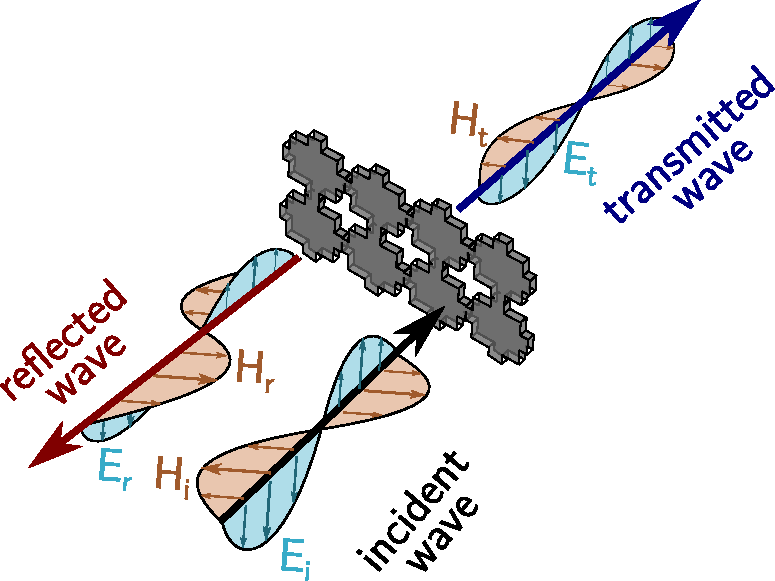
\includegraphics[width=8cm]{img/sim_separating_wave.pdf} \label{fg_separating_wave}\end{figure}

The monitor planes are assumed to be located in vacuum, and at a sufficient distance to eliminate the evanescent waves of the structure simulated. It follows that the vectors of the electric field $\E$, magnetic field $\HH$ and wave vector $\kk$ must a form right-handed triplet. %% TODO reference the M. E. solution
At both monitor planes, the forward and backward wave are linearly superposed as illustrated in Fig. \ref{fg_separating_wave}. Therefore they can be separated by the following relations: 
\begin{equation} 
	\begin{split}
		A^{\text{(in1)}}(f)  := \frac{E_{x}^{(1)}(f) + Z_0 H_{y}^{(1)}(f)}{2}, \quad \quad \quad & A^{\text{(out1)}}(f) := \frac{E_{x}^{(1)}(f) - Z_0 H_{y}^{(1)}(f)}{2}\\
		A^{\text{(out2)}}(f) := \frac{E_{x}^{(2)}(f) + Z_0 H_{y}^{(2)}(f)}{2}, \quad \quad \quad & A^{\text{(in2)}}(f)  := \frac{E_{x}^{(2)}(f) - Z_0 H_{y}^{(2)}(f)}{2}. 
	\end{split} 
\label{eq_separate_ampli}\end{equation}
The constant $Z_0$ stands for the \textit{vacuum impedance}, i.e. ratio of the electric and magnetic field of a freely propagating wave. Its physical value is $Z_0 = \sqrt{\mu_0/\varepsilon_0} = 4\pi c \cdot 10^{-7} \approx 376.7$ $\Upomega$, but in the actual FDTD simulations, the built-in convention of $Z_0 = 1$ was used.
The wave separation result is plotted in Fig. \ref{fg_ampli}.  
\begin{figure}[ht] \caption{Separated amplitudes of the forward and backward waves at the first and second monitor planes 
allow to assess the validity of the results.\\
The incident wave $A^{\text{(in1)}}(f)$ should have smooth spectrum (blue curve), as it is directly generated by the broadband source. The reflected wave $A^{\text{(out1)}}(f)$ (green curve) and the transmitted one $A^{\text{(out2)}}(f)$ (red curve) should be somewhat complementary to each other, since squares of their amplitudes should approximately sum up to the square of the incident wave amplitude, or less in case of losses. \\
The fourth wave $A^{\text{(in2)}}(f)$ should be negligible, as almost all wave energy is expected to be absorbed by the perfectly matched layers at the $z$-faces of the simulation volume. In practice it is nonzero, also due to numerical imprecision and remaining near-field components of the structure. In Fig. \ref{fg_separating_wave}, this relative error in amplitude is less than $10^{-3}$.}  \centering 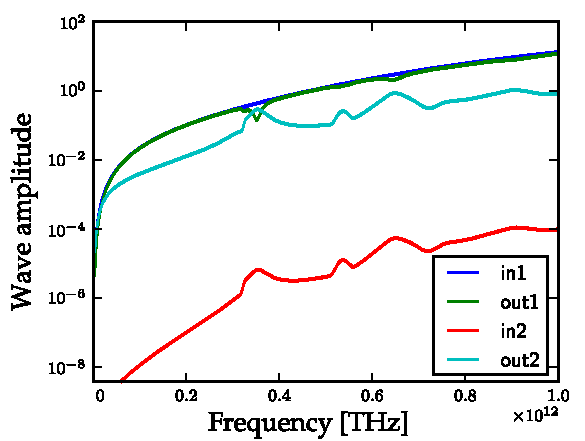
\includegraphics[width=10cm]{img/sim_ampli_debug_band.pdf}\label{fg_ampli} \end{figure} 

Finally, one can easily compute the complex-valued scattering parameters $r(f)$ and $t(f)$ as the ratios of the reflected and transmitted wave amplitudes to the incident wave, respectively:
\begin{equation} 
	\begin{split}
		s_{11}(f) \equiv r(f) := \frac{A^{\text{(out1)}}(f)}{A^{\text{(in1)}}(f)},\\
		s_{12}(f) \equiv t(f) := \frac{A^{\text{(out2)}}(f)}{A^{\text{(in1)}}(f)}.
	\end{split}
\label{eq_sparam}\end{equation}

%}}}
\paragraph{Comparison of simulated and experimental spectra} %{{{

\begin{figure} 
\caption{\textbf{(a)} Electron microphotograph of the STO array (from \cite{nemec2009tunable}), front view, 
\textbf{(b)} dimensions of one unit cell thereof, drawn as the side view}  \centering 
\begin{overpic}[width=.6\textwidth]{img/STOBar_photo.pdf}     \put(0,67) {\textbf{(a)}} \end{overpic}\quad
\begin{overpic}[width=.3\textwidth]{img/EBars_STO_sketch.pdf} \put(1,95) {\textbf{(b)}} \end{overpic}
\label{fg_STO_bar_geom} \end{figure} 

To verify the simulation results against experimental data, we computed $r(f)$ and $t(f)$ for a structure that had been measured in our terahertz laboratory.
It consisted of an array of high-permittivity dielectric bars, cut using a femtosecond laser % todo{what was the laser power and other parameters?
from a 26 $\upmu$m thick strontium titanate (STO) slab \cite{nemec2009tunable}. The periodicity was 96 $\upmu$m and the laser cut width 30 $\upmu$m, resulting in the 66 $\upmu$m width of each rectangular bar as shown in Fig. \ref{fg_STO_bar_geom}. 

The permittivity of STO strongly depends on the temperature, and was not known a priori, so it was chosen as $\varepsilon_r(1\text{ THz}) = 365 + 62\ii$ for the simulation to match the experimental spectra.
\begin{figure} \caption{Experimental transmission $t_{exp}(f)$, compared to numerical reflection $r(f)$ and transmission $t(f)$ for strontium titanate bars of rectangular cross-section $26 \times 66$ $\mu$m, oriented parallel to the electric field. }  \centering 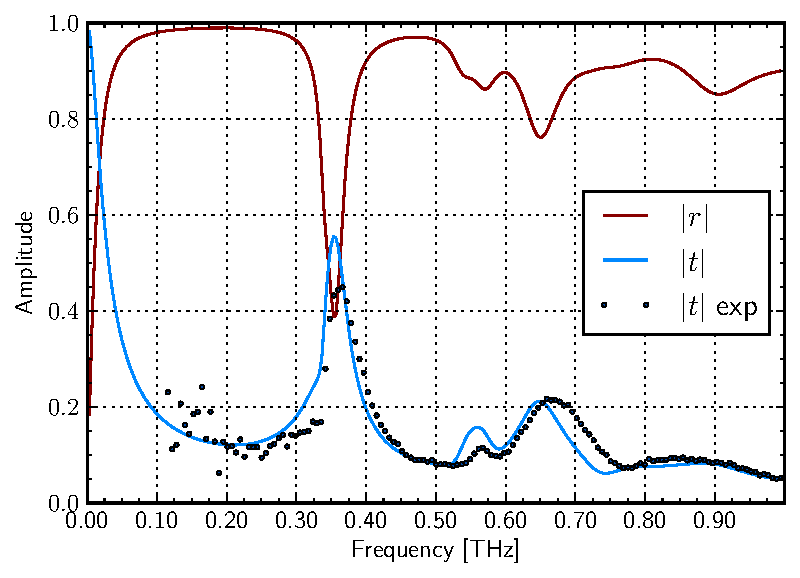
\includegraphics[width=12cm]{img/STObar_rt.pdf} \label{fg_STO_bar_rt} \end{figure} 

	The curves computed using the FDTD simulations are compared to the experimental ones in Fig. \ref{fg_STO_bar_rt}, with a very good match in three well-resolved resonance peaks, and also in the high reflectivity ($|r| > 0.9$) in most of the spectrum which is caused by a great impedance mismatch between the dielectric and the surrounding air.

\begin{figure}[ht] \centering \caption{Parametric scan through the strontium titanate bar width (in micrometers), loss spectra computed as $1-|r^2|-|t^2|$. The bar width of 66 $\mu$m is denoted by the white line. Different modes are joined by black curves and their electric field shapes are drawn above the plot.} 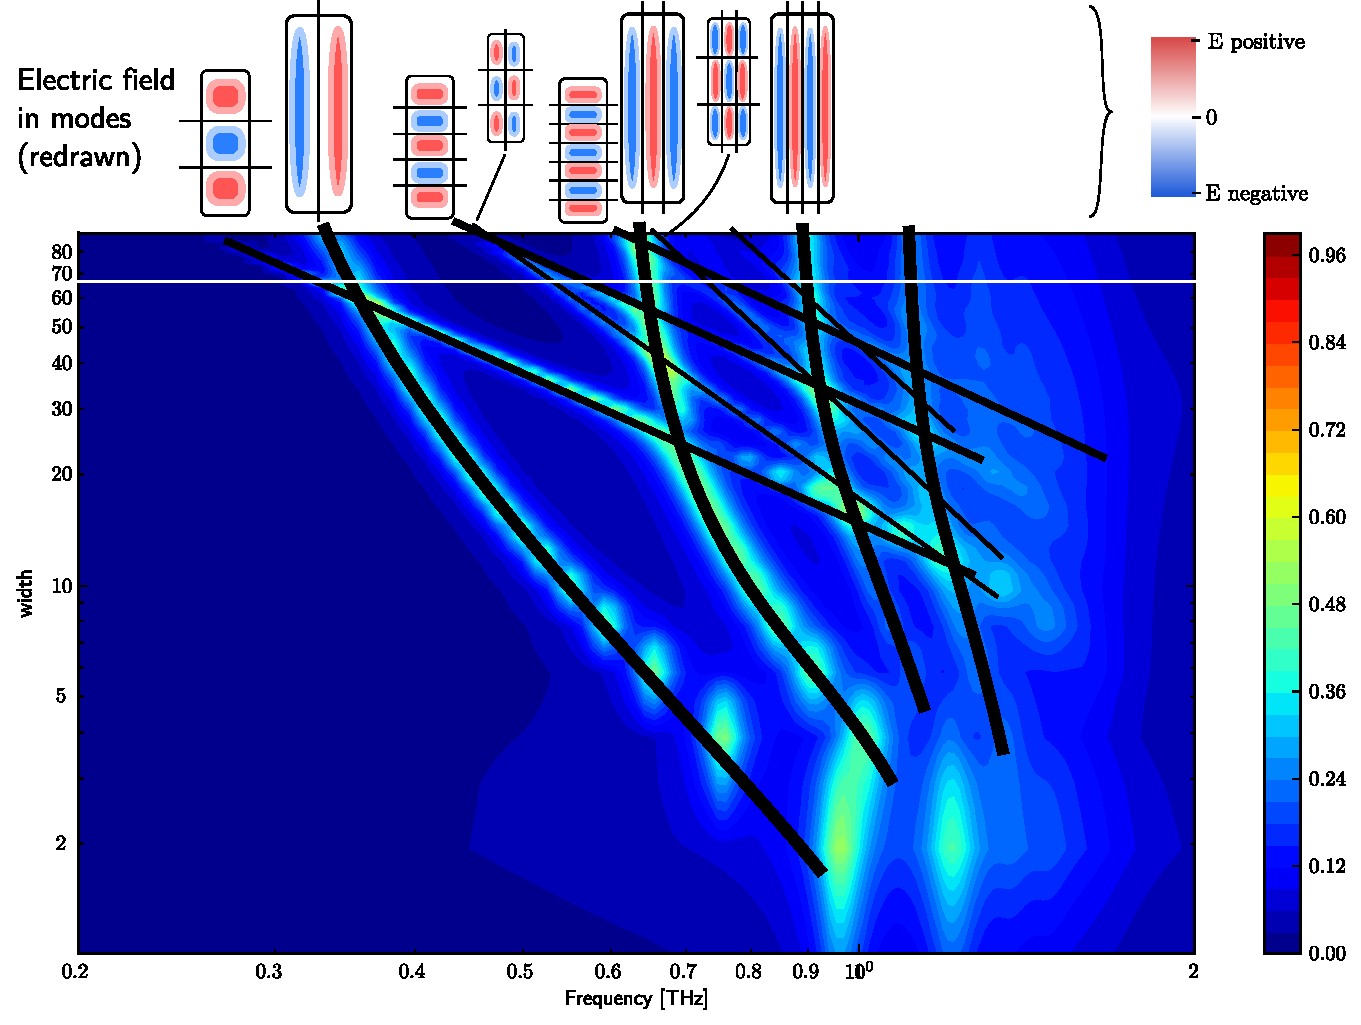
\includegraphics[width=\textwidth]{img/STOBarC_modes2.pdf} \label{fg_STO_bar_modes} \end{figure}
%}}}
\paragraph{Example of a parametric scan with FDTD simulations} %{{{
To briefly illustrate further possibilities of the numerical simulations, we scanned the relative width of the STO bar, and computed the relative energetic loss in the structure given by $1-|r^2|-|t^2|$. Each loss peak can be clearly associated with one resonant mode in the dielectric, as shown in Fig. \ref{fg_STO_bar_modes}. Only modes with a mirror symmetry in the transverse direction ($y$-axis) couple to the wave; the remaining antisymmetric modes would manifest themselves at oblique incidence only.

The two-dimensional scan can reveal further information about the underlying physics. Most importantly, it is clear that the resonance frequency of the modes has a different sensitivity to the bar width. Note that both vertical and horizontal axes are logarithmic, so the power dependence can be directly estimated from the slope of the line. 

It can also be seen from Fig. \ref{fg_STO_bar_modes} that for the bar width close to 66 $\upmu$m, which is indicated by the horizontal white line, two modes cross-over in frequency. Namely, one of these is a narrow mode with nodal planes almost parallel to the wave propagation, while the second is much broader one with one nodal plane centered inside the dielectric slab volume. This explains why the first resonance in Fig. \ref{fg_STO_bar_rt} has an obviously asymmetric shape, both in the simulated and experimental spectra. 

The overlap of two modes differing by both spectral width and resonance frequency forms a typical \textit{Fano resonance} shape, which would be probably experimentally observed if the losses were lower.
A more elaborate discussion of periodic structures composed of dielectric bars/rods oriented either along the electric or the magnetic field will follow in the Sections \ref{sect_diel_rods_mag} and \ref{sect_diel_rods_el}.
%}}}
\paragraph{Retrieval of the effective parameters} %{{{
%So far, only the amplitude and phase of frequency-dependent reflectance $r(f)$ and transmittance $t(f)$ for a finite number of metamaterial cell layers were determined. 
Complemented with the cell thickness $d$, the spectra of the frequency-dependent reflectance $r(f)$ and transmittance $t(f)$ can serve as inputs for the s-parameter method,  \cite{smith2002determination, smith2005electromagnetic} \cite[pp. 51-55]{shalaev2010book}. The expression for the effective index of refraction is
\begin{equation} \Neff = \frac{\pm \arccos\left(\frac{1 - r^2+t^2}{2 t}\right) + 2\pi\,m}{k d}, \label{eq_Neff} \end{equation}
where nor the integer-valued branch index $m\in \mathbb{Z}$, nor the sign of the solution are a priori known. For the effective impedance, the sign is also ambiguous: 
\begin{equation} \Zeff = \pm \sqrt{\frac{(1+r)^2 - t^2}{(1-r)^2 - t^2}}. \label{eq_Zeff} \end{equation}

%}}}
\paragraph{Search for the correct solution} %{{{
From Eqs. (\ref{eq_Neff}) and (\ref{eq_Zeff}) it follows that the correct solution depends on three discrete-valued functions of frequency, i.e. the sign of $\Neff(f)$, the sign of $\Zeff(f)$ and the branch index $m(f)$, which have to be determined during computation.  We identified the following criteria for selection of exactly one of infinitely many solutions:
\begin{enumerate}
	\item{Passivity with regards to the wave propagating through the structure requires the \textit{imaginary} part of refractive index be non-positive: 
		 \begin{equation} \Neff''(f) \leq 0 \quad \forall f\in \mathbb{R} \label{eq_Neff_pass}\end{equation}
		 } 
	 \item{Passivity with regards to the wave reflected from the structure interface requires the \textit{real} part of refractive index be non-positive, too: 
		 \begin{equation} \Zeff'(f) \leq 0 \quad \forall f\in \mathbb{R} \label{eq_Zeff_pass}\end{equation}
		 } 
	 \item{Causal response of the sample requires specific relation between the real and imaginary parts of $r(f)$, $t(f)$ and of effective parameters $\Neff(f)$ and $\Zeff(f)$, when substituted for the function $F(\omega)$:
		 \begin{equation} 
F'(\omega) = \int_{-\infty}^{+\infty}  \frac{-2\ii}{\omega - \Omega} F''(\omega) \,\mbox{d}\Omega  \equiv  \left[\frac{-2\ii}{\omega}\right]\,\ast\,F''(\omega). \tag{\ref{eq_kkresult} \again}\end{equation} 
Perhaps the most familiar consequence of this criterion is the requirement of continuity for $\Neff(f)$ in all structures with nonzero losses.
		 } 
\end{enumerate}
Note that in the papers that use different complex convention, i.e. $e^{-\ii\omega t}$, both passivity conditions use the opposite sign. This does not apply to the kernels of the Fourier nor Hilbert transforms.

%}}}
\paragraph{Effective $\Neff'$ retrieval based on unambiguous complex arccosine} %{{{
\begin{figure} \centering \caption{\textbf{(a)} Real and \textbf{(b)} imaginary parts of the arccosine of complex argument $\upsilon$. Branch cuts are denoted with thick lines. The thick curve shows a possible trajectory of  $\upsilon(f)$ (upon a frequency variation), which intersects the branch cuts in points marked as R, L.\\ \textbf{(c)} From top to bottom: an example function  $\upsilon(f)$, its ordinary arccosine, example branch and sign choices ensuring the continuity of the arccosine function, and the continuous version of $\arccos_{\mathrm{c}}(\upsilon)$, as determined by the algorithm described.} 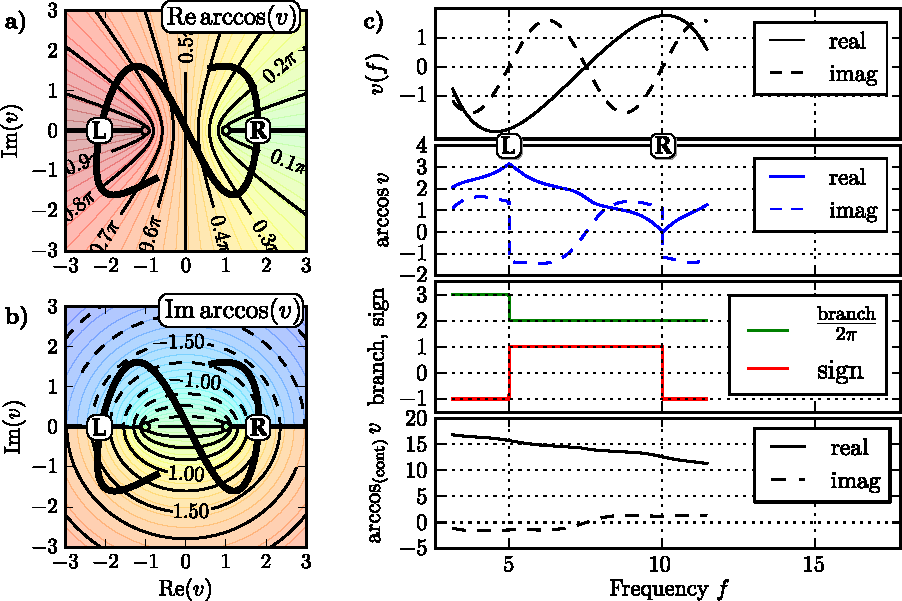
\includegraphics[width=16cm]{img/continuous_arccos/continuous_arccos_new.pdf} \label{fg_arccos}
\end{figure}

We wrote a custom procedure to select the correct solution automatically on pure mathematical basis. To our knowledge, it was not described in any of previously published papers. Alternative approaches are briefly discussed in the following section.

The ambiguity in Eqs. (\ref{eq_Neff}, \ref{eq_Zeff}) results from the fact that the inverse functions of arccosine and square root are not injective mappings \cite{simovski2009material}:
\begin{equation} \cos x = \cos (-x) = \cos(x+2\pi) \quad  \forall x\in\mathbb{C}, \label{eq_noninjN}\end{equation}
\begin{equation} x^2 = (-x)^2 \quad \forall x\in\mathbb{C}. \label{eq_noninjZ}\end{equation}
%Although the range of values for arccosine and square root are defined uniquely in mathematics, the retrieval algorithm described here extends these functions to yield different values to ensure continuity.
Since the temporal records of the fields are exponentially decaying functions, the reflectance  $r(f)$ and transmittance spectra $t(f)$ must be continuous. 
It is assumed that for any realistic structure with nonzero losses, the transmission never passes exactly through the complex zero, and the arccosine argument from Eq. (\ref{eq_Neff})
\begin{equation} \upsilon(f) = \frac{1-r^2+t^2}{2t},   \label{eq_upsilon}\end{equation}
is also a continuous complex function. Any discontinuities in the retrieved spectra of $\Neff'(f)$ may therefore arise exclusively at the discontinuities of the arccosine function in the complex plane.

To ensure overall continuity of $\Neff$ in Eq. (\ref{eq_Neff}), it is therefore necessary to identify the two \textit{branch cuts} of arccosine in the complex plane, as illustrated in the left subplots of Fig. \ref{fg_arccos}a,b. Different measures must be taken for the sign and branch index $m(f)$ to ensure continuity:
\begin{enumerate}
\item{
If, by increasing the frequency, the arccos argument $\upsilon$ passes through the right branch cut at $\upsilon' > 1, \upsilon'' = 0$ (point "R" in Fig. \ref{fg_arccos}c), the real part of arccos$(\upsilon)$ touches zero, whereas its imaginary part is non-zero and changes its sign. The direction given by the sign of $d\upsilon'/df$ does not play role. The continuity is achieved if, from this frequency on, one reverses the sign of the arccos term . 
} 
\item{
		At the left branch cut (the "L" point in Fig. \ref{fg_arccos}c), i.e., for $\upsilon' < -1, \upsilon''=0$, where the imaginary part of $\arccos(\upsilon)$ experiences again a step-like change of the sign, but the real part touches the value of $\pi$. To restore the continuity, the sign reversal must be also accompanied by a change of the branch index. . 
} 
 \end{enumerate}

%}}}
\paragraph{Effective impedance retrieval} %{{{
The sign of the square root function is similarly chosen such than $Z$ is a continuous function of frequency. Probably the simplest approach is to express the square root argument in Eq. (\ref{eq_Zeff}) in polar nonation, i.e., as its real-valued modulus and its angle in the complex plane. The angle can be easily ensured to be a continuous function by shifting it by $\pm 2\pi$ at any discontinuity.

Using the \textit{Moivre theorem}, the square root is then computed by halving the angle of the argument, and computing the square root of its real-valued modulus. Both operations are safe in terms of maintaining the continuity.

The particular implementation of continuous arccosine and square root retrieval can be found online in Ref. \cite[\texttt{effparam.py} file]{dominec2014_meep_metamaterials}.

%}}}
\paragraph{Initial branch and sign choices}%{{{
Next, it is necessary to establish the sign and branch index of $\Neff$ and the sign of $\Zeff$ at the starting point of the spectrum. One can assume that for very low frequencies below any individual resonance, also the Bloch wave vector tends to zero $K\rightarrow 0$. In case of conductive structures, the spectrum starts with a plasma-like band gap at low frequencies, leading to evanescent wave with vanishing wavenumber as well.

Whenever the spectra of $r(f)$ and $t(f)$ are computed using the Fourier transform, they are known for very low frequencies  nd the selection of the branch is thus easy.

The remaining step is to establish the signs of $\Neff$ and $\Zeff$, using the aforementioned rules of the metamaterial passivity.

%}}}
\paragraph{Computing effective parameters for a 1-D photonic crystal}%{{{
The described algorithm was proven to work reliably with most structures. However, it is sensitive to numerical errors 
when the arccosine argument $\upsilon(f)$ from Eqs. (\ref{eq_Neff}, \ref{eq_upsilon}) passes 
near the points $(-1+0\ii)$ and $(1+0\ii)$, that is, near the ends of the branch cuts of the complex arccosine.

Unfortunately, it was observed that $\upsilon(f)$ touches these points in the spectra of planar slabs of lossless dielectric. Correct retrieval of spectra for this particular structure requires that even in these points, the curve is processed as if it had crossed the branch cut. 

Otherwise, the retrieved spectrum of $\Neff(f)$ remains continuous, but at higher frequencies it ceases to make physical sense. Its imaginary part acquires the wrong sign in the band gaps, breaking the passivity criterion. Simultaneously, its real part decreases with frequency in the next photonic band, which breaks the Kramers-Kronig relations of Eq. (\ref{eq_kkresult}) and would be a sign of negative group velocity occurring without significant dispersion. Thus, this error can be easily notified, and with further programming it cold be combined with the verification against the Kramers-Kronig relations.

This is the only issue which arises from the described effective-index retrieval algorithm known to the author. It has proven to be efficiently resolved by introducing moderate losses into the structure and/or artificially shifting the branch-cut detection points to be slightly closer to the complex zero, e.g. to $(-0.999+0\ii)$ and $(0.999+0\ii)$. In many cases, the wrong detection of the branch was resolved simply by multiplying the recorded fields by the smooth window function from Eq. (\ref{eq_envelope}).

%}}}
\paragraph{Summary of the scattering-parameter method}%{{{
The scattering-parameter method is the most widely used setup for the effective parameter retrieval. It stands out among other setups by relying on the amplitudes of the reflected and transmitted waves only, without any inspection of the fields inside the unit cell. It is also efficient, since it requires single time-domain simulation to retrieve the full spectrum of effective parameters. The wave is let to freely propagate through the structure, and afterwards the retrieval algorithm determines the wavenumber at each frequency component of the incident wide-band pulse. The frequency $\omega$ represents the input, and the wavenumber $K(\omega)$ is one of the outputs.

However, the scattering-parameter method also has its weaknesses. Perhaps its greatest weakness is that it does not explicitly fail in cases it is not supposed for; or, as stated in Ref. \cite{markel2013current}:
\begin{cite} \textit{Of course, a refractive index per se (generally, tensorial and dependent on the direction of the Bloch wave vector) can always be formally introduced for a Bloch wave.} \end{cite}
Great care must be paid whether the retrieved values of effective parameters make any physical sense whatsoever, or are just a confusing output of an algorithm used outside its scope. The majority of the possible issues was mentioned above:
\begin{enumerate}
		 \item{It is intrinsically imprecise, because the evanescent fields of most structures are influenced by the free space in front the unit cell and behind it. This issue can be neglected if nearly all of energy is transferred by the radiated wave, in which case the metamaterial is sometimes described as a \textit{Bloch lattice} \cite{simovski2007bloch, andryieuski2012bloch}. In other cases, usually in dense or metallic structures, a significant amount of energy is transferred by the near-field coupling, and it can be demonstrated that the effective parameters retrieved by this method strongly depend on the number of layers \cite{rockstuhl2008transition,andryieuski2010homogenization} which renders the approach invalid.
			 } 
		 \item{Another source of the error is the fact that the monitor planes detect also the near field, requiring to add a distance between the structure and the monitor planes.} 
		 \item{Although we devised a relatively robust computation of effective parameters, the current implementation is still sensitive to numerical errors when spectra of lossless dielectric slabs are computed.} 
		 \item{The method requires the structure to be symmetric with regards to the wavevector $\KK$, since it attempts to approximate it by effective parameters that leave no degree of freedom for possible asymmetry. An example of an asymmetric structure was discussed in Ref. \cite{smith2005electromagnetic}, where it was concluded that
 \begin{displayquote} \textit{ so different are the two solutions for $\Zeff$ for the asymmetric structure that in general the assignment of values of $\eeff$ and $\meff$ to the composite becomes counterproductive} 
 \end{displayquote}
 In the view of the author of this thesis, also the retrieved $\Neff$ in Fig. 7c of Ref. \cite[p. 036617-9]{smith2005electromagnetic} can be reasonably interpreted if and only if the structure is symmetric. 
			 }
	     \item{Perhaps the most fundamental limitation of this method comes from its principle of retrieving the wavenumber at a given frequency. For periodic structure which exhibits strong enough spatial dispersion, more than one wavenumber exist at a single frequency as shown in Figs. \ref{fg_dcll_nl}. For any frequency from such a problematic range, the detected effective parameters depend on the unknown ratio of energy coupled to either of the waves. Therefore, the method is inapplicable for structures with a strong spatial dispersion. This effect is illustrated in the Results section (e.g. in Fig. \ref{fg_cdh2}).
			 }
\end{enumerate}

%}}}

\subsection{Current-driven homogenisation} 
\paragraph{Principle} %{{{
When more than one wavevector $\KK$ corresponds to a given frequency,  
a different approach to the effective-parameter retrieval must be used, for which the wavevector $\KK$ becomes the input, and the corresponding frequencies $\omega_{1\ldots\infty}(K)$  at the dispersion curves are returned as the output. 
This section describes the \textit{current-driven homogenisation} (CDH), in which whole simulation is computed exclusively with a single wavevector $\KK$, and the dispersion curves are reconstructed from multiple simulations differing by the wavevector. 

In this thesis, the method is described in its simplest form. More elaborate implementation is discussed in Refs. \cite{silveirinha2007metamaterial}, \cite{fietz2010current} and \cite{fietz2011homogenization} and enables to recover all 36 parameters that describe the influence of the fields ($E_x$, $E_y$, $E_z$, $H_x$, $H_y$, $H_z$) to the displacements ($D_x$, $D_y$, $D_z$, $B_x$, $B_y$, $B_z$), taking into account also possible anisotropy and bianisotropy.

%}}}
\paragraph{Bloch-periodic boundaries for arbitrary wave vector} %{{{
In CDH, the unit cell is simulated as being placed in an infinite lattice, neighbouring with the same cells of size $a$ in all three dimensions. To emulate such lattice in a simulation of a single cell, all the faces of the unit cell have to be set Bloch-periodic, i.e., set to copy the field from the opposite face.

Exact copying of the fields from one side to another would require the wavevector of the Bloch wave to be strictly $K_{xyz} \in 2\pi m/a_{xyz}$, which is, however, the known condition for a photonic band gap. Since we are mostly interested in computing the wavenumber inside photonic bands, the periodic boundaries have to allow for an arbitrary phase shift before the fields are copied:
\begin{equation} E(\rr + a_x\mathbf{x}/2) \quad\rightarrow\quad  e^{-\ii K_x a_x}\; E( \rr - a_x\mathbf{x}/2), \label{eq_phaseshiftp}\end{equation}
	where $\mathbf{x}$ is the unit vector along the x-axis, and $a_x$ are the unit cell size along this axis. The unit cell is assumed to be centered around the $x=0$ point, thus $x=\pm a_x/2$ denotes the point at the boundary, and similarly for other axes.

Positive phase advance is applied when copying the fields parallel to the x-axis, and negative phase retardation is applied when simultaneously copying the fields in the opposite direction:
\begin{equation} E(\rr - a_x\mathbf{x}/2)  \quad\rightarrow\quad  e^{+\ii K_x a_x}\; E(\rr + a_x\mathbf{x}/2). \label{eq_phaseshiftn}\end{equation}
A similar field-copying procedure is repeated in each simulation step for all remaining axes, $\mathbf{y}$ and $\mathbf{z}$, in the case of a 3-D simulation. 

%}}}
\paragraph{Single-wavevector source}%{{{
In order to excite the simulation volume with a single wavevector $\KK$ which complies to the Bloch-periodic boundary conditions imposed, the source volume must expand over the whole unit cell and acquire a correct harmonic modulation of its complex amplitude. While this task appears impossible by experimental techniques, it is straightforward in the FDTD simulation. The source is typically designed to be a complex-valued electric current with a given amplitude:
\begin{equation} \mathbf{J}(\rr, t) := \mathbf{x} \, e^{-\ii \KK\cdot \rr} \,j(t), \label{eq_}\end{equation}
	where $\mathbf{x}$ determines the default polarisation of the electric field and $j(t)$ is the temporal profile of the source.

Excitation of the structure with this kind of the source gave the current-driven homogenisation its name. Unlike the scattering-parameters method, in CDH the source volume coincides with the entire unit cell volume. An attempt of visualisation of this minimalistic simulation setup is in Fig. \ref{fg_fdtd_cdh}. 
\begin{figure}[h] \centering \caption{Current-driven homogenisation setup consists of a single unit cell with all faces set to be Bloch-periodic, with appropriate phase shift between the corresponding pair of faces. One example of the real part of the spatially varied source amplitude is sketched along the unit cell edge as the green-filled curve.} 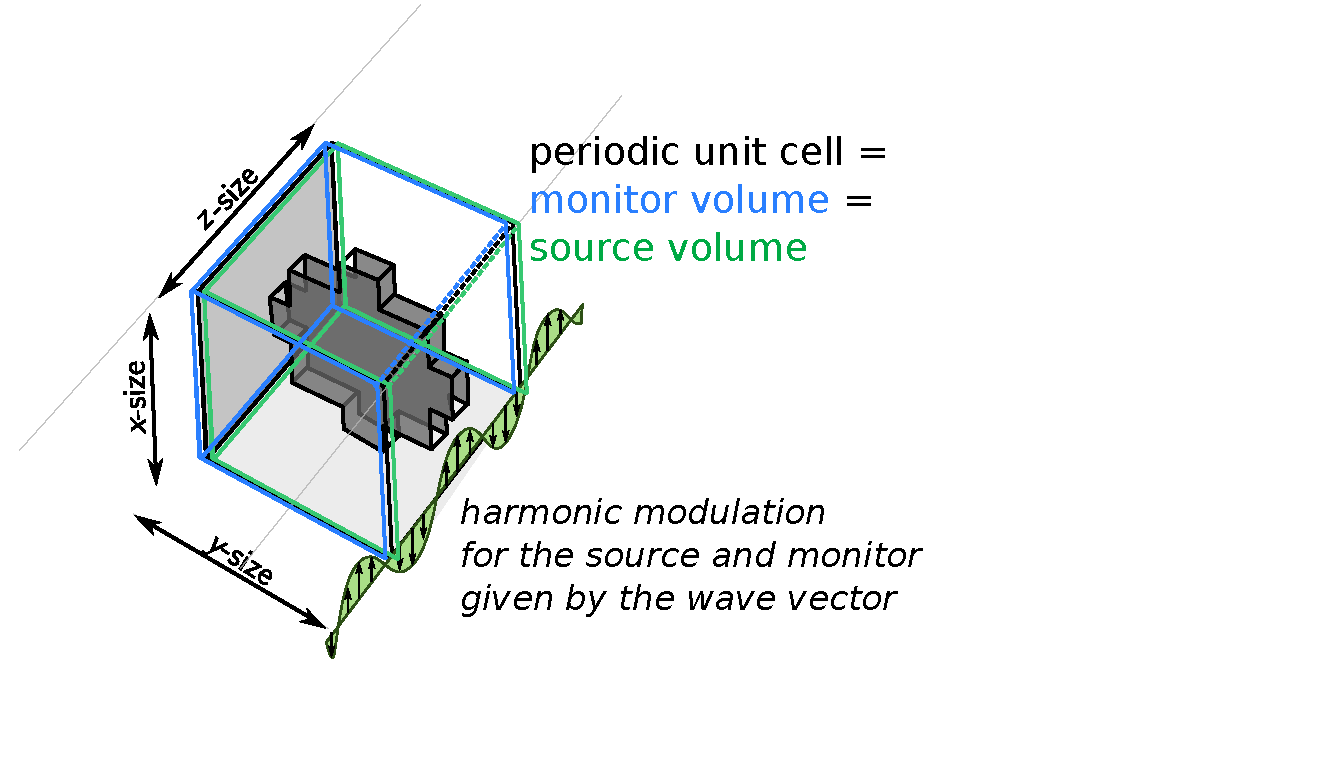
\includegraphics[width=.5\textwidth]{img/cdh_geometry.pdf}  \label{fg_fdtd_cdh} \end{figure} %% 
%}}}
\paragraph{Temporal profile of the source}%{{{
With the wavevector restricted to a single given value, it is necessary to excite and detect as many corresponding modes of the structure as possible. Therefore, a short and broadband temporal source profile could be reused from the scattering parameter method. 

Unlike the scattering-parameters method, CDH can not easily detect the spectral profile of the exciting field, and the retrieved fields can not be normalized against it. To maintain an approximately flat source amplitude over a wide part of the specturm, a nontrivial temporal shape of the source was designed, tested and submitted to the MEEP simulation developer site \cite{} online:
\begin{equation} 
	j(t) := w_{BN}(t)\, \left[\mathrm{Si}(2\pi f_1 t) - \mathrm{Si}(2\pi f_2 t) \right]
\label{eq_}\end{equation}
where the transcendent sine-integral function introduces the flat-top rectangular spectrum of the wave radiated from the source:
\begin{equation} \mathrm{Si}(t) = \int_0^t \frac{\sin \tau}{\tau} d\tau, \label{eq_Si}\end{equation}
	The electric field radiated by a source is proportional to the temporal derivative of the current $j(t)$ \cite{ab-initio}, therefore the sine-integral must be used to obtain the field shape of $E_x\propto \sin(t)/t$, which is known to have a rectangular flat-top spectrum.

If the source amplitude had an infinite duration in time, its spectrum would form a perfect rectangular function. However, clipping the temporal duration of the source results in spectral artifacts, as was already described on the page \pageref{convolringing}.
The artifacts can be very efficiently suppressed by multiplying the source by the \textit{Blackmann-Nutall window}  function
\begin{equation} 
\begin{split} 
	w_{BN}(t) :=\; & 0.3635819 + \\
			 &+ 0.4891775\,\cos\frac{2\pi(t-t_c/2)}{t_c} + \\
			&+ 0.1365995\,\cos\frac{4\pi(t-t_c/2)}{t_c} + \\
			&+ 0.0106411\,\cos\frac{6\pi(t-t_c/2)}{t_c} \quad \text{for } t\in\langle0, t_c\rangle, \\
	w_{BN}(t) :=\;& 0 \quad \text{otherwise.}
\end{split} 
\label{eq_wBN}\end{equation} %% TODO verify again
Since $w_{BN}(t)$ has finite support in time, but particularly fast decaying wings in its spectrum, it ensures relatively steep edges of the nearly rectangular spectrum of the source.

%}}}
\paragraph{Field monitor and identification of the dispersion curves}%{{{
The detection of the fields is defined in a way similar to the definition of the source. In each timestep, the electric field $E_x(\rr,t)$ is sampled in multiple points through the unit cell. As each of the points could have a different phase, the values are divided by $e^{-\ii \KK\cdot \rr}$ before they are averaged.

After the simulation ends, the single record of cell-averaged $E_x$ is processed to identify the set of frequencies $\omega_m(\KK)$ at which $E_x$ exhibited a ringdown. For example, if the cell is empty vacuum, the source with wavevector $\KK$ can only excite a wave at the frequency $\omega = Kc$. All other combinations of $(\omega, \KK)$ are off the dispersion curve (known also as the light line in vacuum) and no solution of Maxwell equation exists for them. Although the source can create temporary evanescent fields even at such "off-shell" combinations, the evanescent-field energy is immediately returned back to the source. 

The same holds for any kind of structure placed in the unit cell: the energy persists to the end of the simulation only at frequencies $\omega_m(\KK)$ that lie at one of corresponding dispersion curves. An intuitive way of detecting such frequencies would be to compute the Fourier transform of the recorded averaged field $E_x$ and identify the peaks in the resulting spectrum. The resolution of the Fourier transform is nonetheless proportional to the time record, and it is inefficient for the task of accurately recognizing the frequencies of a small number of damped oscillations.

A more advantageous algorithm for recognition of oscillations is the \textit{filter diagonalisation method} (FDM), originally  developed in 1990 for analysis of experimental spectra and the nuclear magnetic resonance waveforms in particular \cite{mandelshtam1997harmonic, chao2002comparative}. Unlike Fourier transform, FDM does not require the oscillators to decay before the temporal record ends; on the contrary, it appears to work even more reliably when supplied with several tens of the oscillation periods at most. Using FDM, the simulation time could be shortened several times.

%}}}
\paragraph{Advantages over the scattering-parameters method}%{{{
Using CDH resolves some of the issues of the s-parameters method, namely 
\label{cdhadvantages}
\begin{enumerate}
\item{It simulates the unit cell embedded from all sides in the lattice, and there is no problem with the evanescent fields sensing free space as it was in the s-parameter method.} 
\item{Retrieval of the dispersion curves is not much sensitive to the actual field amplitude, but rather to the frequencies detected in its ringdown. The shape of dispersion curves is less distorted by any possible error during the scattered field detection.} 
\item{Since the wavevector is given before each simulation, no issues with wrong branch detection can flip or otherwise distort the dispersion curves.} 
\item{Also the requirements to the structure symmetry are weaker. In general, the structure is not required to have any symmetry plane perpendicular to the wavevector. Other kinds of lower symmetry may lead to bianisotropic behaviour, which would require more sophisticated detection of the waves, though.}
\item{Last but not least, CDH in comparison with the s-parameters method inherently takes into account even a very strong spatial dispersion. All additional waves are detected correctly.}
\end{enumerate}

CDH also has more general applicability. It can easily operate with arbitrary orientation of the wavevector $\KK$. It can even excite longitudinal waves in the structure, and naturally retrieve their dispersion curves which can also depend on $\KK$ due to the spatial dispersion. 

%}}}
\paragraph{Weaknesses compared to the scattering-parameters method}%{{{
The downside of CDH, as implemented in this thesis, is mainly in the fact that it provides less information than the s-parameter method: 
\begin{enumerate}
\item{It does not compute the effective impedance $\Zeff$ at all, and it is questionable whether $\Zeff$ could be computed if also the averaged magnetic field $H_y(\rr, t)$ was recorded. } 
\item{On the one hand, CDH reliably computes the dispersion curves, and the corresponding set of $\omega_m(\KK)$ functions could be inverted into $\KK(\omega)$ and, for propagation along an optical axis (c.f. page \pageref{indexofrefraction}), also into $\Neff(\omega)$. On the other hand, it does not give any information on the topology of nodal planes, and which branch of $\Neff(\omega)$ would be selected by the s-parameter method. } 
\item{We did not manage to obtain any useful information related to the imaginary part of $\Neff$ -- about the structure losses, field decay in photonic band gaps, and its behaviour outside the dispersion curves in general.}
\end{enumerate}
Other downsides relate to the practical implementation, and arguably are the reason for its rarer use in the literature.
\begin{enumerate}
\item{A comparable task in CDH is more computationally intensive than in the s-parameters method. For a single set of dispersion curves, several tens of simulations with different $\KK$ are needed. After they are run, a postprocessing script must analyze all recorded fields and assemble the dispersion curves. }
\item{Naturally, CDH can hardly be employed in an experiment, since it inspects the field in multiple points inside the structure simultaneously. }
\end{enumerate}
In spite of these limitations, the simplified implementation of CDH for this thesis remains an important complement to the s-parameter method. 

%}}}

\subsection{Other effective parameter retrieval methods}      % complement?
\paragraph{Extensions of the scattering parameters method} %{{{
Various modifications to the scattering parameters method were proposed, in particular with connection to the homogenisation of metamaterials. One modification makes it robust against the experimental error in the reflectance phase \cite{chalapat2009wideband}. % Wideband reference-plane invariant method for measuring electromagnetic parameters of materials
Another solution to the issues connected with experimental measurement of the reflectance was employed during the preparation of this thesis \cite{nemec2012resonant}. It involved a slight modification to the experimental setup, and thus it is described in the experimental chapter (pp. \pageref{srtm}--\pageref{srtm2}).

Some of the modifications apply to the effective parameters retrieval only, and no change is made to the way how  the scattering parameters $r(f)$ and $t(f)$ are obtained.
Not knowing the correct branch of the index of refraction is equivalent to using the folded dispersion curves (cf. Par. \ref{par_disp_curv_per}), %% TODO refer to the theory
so the postprocesing of FDTD data can also be viewed as a specific, nontrivial way of \textit{unfolding} the dispersion curves. This task appears to have been often done manually, particularly in earlier papers \cite{smith2002determination}. An approach based on iterative fitting which avoids abrupt discontinuities in $\Neff'(f)$ has been published \cite{chen2004robust}, but the author conjectures that, from its very nature, it would become unstable whenever a localized resonance introduces fast changes of $\Neff'(f)$, which can be found e.g. in Fig. \ref{fg_CutWires_wireradius1u_cutwidth_comparison}. Manually assisted approaches present the risk of affecting the resulting effective parameters with unjustified subjective expectations.

A more elegant method was published in 2010 by Szabo et al. \cite{szabo2010unique} and relies on the inherently unambiguous knowledge of $\Neff''(f)$. It uses the Hilbert transform introduced in Eq. (\ref{eq_kkresult}) to recover $\Neff'(f)$ from $\Neff''(f)$. 
However, from our own experience, applying this integral transform to a finite part of spectrum introduces not only an arbitrary constant offset, but also slow continuous distortion of the $\Neff'(f)$ curves, thus needing a nontrivial compensation.

The discussion in this thesis is restricted to the near-perpendicular wave propagation, since it is assumed the optical axis is also perpendicular to the interface. In Ref. \cite{menzel2008retrieving}, Eqs. (\ref{eq_Neff}, \ref{eq_Zeff}) were generalized also for oblique incidence. Note that for retrieving the effective index of refraction one must establish whether it makes any physical sense at all, i.e., whether the structure is either isotropic, or at least whether the angle of refraction is parallel to its optical axis (see page \pageref{indexofrefraction}).

In Ref. \cite{li2009determination}, % Determination of the effective constitutive parameters of bianisotropic metamaterials from reflection and transmission coefficients 
the scattering parameter method was extended also to the bianisotropic behaviour of structures with reduced symmetry, and other approaches can be found \cite{andryieuski2010homogenization} in the recent literature.

%}}}
\paragraph{Averaging of the fields} %{{{
With the scattering parameters method, $\Neff(f)$ and $\Zeff(f)$ are retrieved first using the amplitudes of the reflectance and transmittance.  were computed later. The  local effective permittivity $\eeff(f)$ and permeability $\meff(f)$ can be  computed using  Eqs. (\ref{eq_dispeqN}) and (\ref{eq_Z}), but are considered valid only when $|\Neff'| \ll 2\pi/a$, i.e., when the unit cell size $a$ is much less than the Bloch wavelength.

The effective parameters $\eeff(f)$ and $\meff(f)$ can however be computed directly by exciting a unit cell of the structure, averaging both the fields ($\E$, $\HH$) and the displacements ($\D$ and $\B$), and dividing the respective displacement by the field. The method is described in Ref. \cite{smith2006homogenization}, where also numerical examples are given. 

%As expected, when $|\Neff'| \not\ll 2\pi/a$ the value of $\eeff$ for wire array retrieved by this averaging method deviates from that one retrieved by the s-parameters method \cite[Fig. 5]{smith2006homogenization}. The author believes that none of methods attempting to homogenize the structure by the local parameters, $\eeff(f)$ and $\meff(f)$, can be exact.

%%% Andriy2010: "Field averaging [15-16]. In this case the fields (E, D, H, B) in a unit cell are averaged on some surfaces and lines and the effective properties are found according to material relations D = İ 0 İE and B = μ 0 μH.  Determining appropriate surfaces and contours is a non-trivial problem especially when optimizing 3D MTM structures."
%D.R. Smith and J.B. Pendry, Homogenization of metamaterials by field averaging (invited paper), Journal
%of the Optical Society of America B, vol. 23, pp. 391-403, Mar. 2006.
%J. Lerat, N. Malléjac, and O. Acher, Determination of the effective parameters of a metamaterial by field
%summation method, Journal of Applied Physics, vol. 100, p. 084908, 2006.

% TODO read: http://scholar.google.cz/scholar?q=Tsukerman+2011++of+metamaterial+Rigorous+Whithey+interpolation&btnG=&hl=cs&as_sdt=0%2C5

%}}}
\paragraph{Bloch-mode analysis} %{{{
A \textit{single-interface} method has been proposed \cite{yang2010retrieving} %Retrieving the effective parameters of metamaterials from the single interface scattering problem
that analyzes only the field behaviour at the interface of a semi-infinite structure.  
The fields in the structure are computed and decomposed into discrete modes of the Bloch wave. The method attempts to recognize a dominant Bloch mode for which the wavevector $\KK(\omega)$ is deduced.
%\cite{yang2010retrieving}LISTS: "various numerical techniques have been developed, including field averaging, 7 Bloch mode approaches, 8–10 multipole
%expansion, 11,12 and inversion of scattering parameters."
\cite{zhang2006optical} % Optical negative-index bulk metamaterials consisting of 2D perforated metal-dielectric stacks
\cite{rockstuhl2008light} %Light propagation in a fishnet metamaterial

When no mode is clearly dominant, this method naturally can not be used. In such a case, even the scattering parameter method fails, but its limitations of applicability are less obvious than with the \textit{single-interface} method. Failure of the scattering parameter method can be observed as contradictory results \cite{rockstuhl2008transition} from simulations of different numbers of unit cells.
In Ref. \cite{paul2011reflection} %Reflection and transmission of light at periodic layered metamaterial films
it is argued that the existence of one dominant mode is the prerequisite necessary for the structure to be viewed as homogeneous. Refs. \cite{paul2011reflection,andryieuski2012bloch} apply the Bloch-mode analysis approach is applied to particular structures. A direct numeric evaluation of amplitudes of the different modes in 1-D photonic crystals can be found in 
\cite{mortensen2010unambiguous}. % On the unambiguous determination of effective optical properties of periodic metamaterials: a one-dimensional case study

%\cite{smigaj2008validity} %PDF? Validity of the effective-medium approximation of photonic crystals

%}}}
\paragraph{Wave phenomena} %{{{
% (skip this?) B. Popa and S.A. Cummer, Determining the effective electromagnetic properties of negative-refractive-index metamaterials from internal fields, Physical Review B, vol. 72, p. 165102, Oct. 2005

In the \textit{Wave propagation retrieval method}, proposed in Ref. \cite{andryieuski2010homogenization},
the wave impinges a thick, ideally semi-infinite, volume of the periodic structure. Since there are no repeated reflections from the second interface, the averaged field amplitude is assumed to have an exponential nature: $E(z) \propto e^{-2\pi i f \Neff/c}$, and thus $\Neff$ can be reconstructed using a complex logarithm.

Like in the s-parameters method, the function of $K(\omega)$ can be resolved in a single run by using a broad band pulse. Like in the current-driven homogenisation,  the fields need to be sampled inside the structure. 
% unambiguously retrieves bulk parameters; but there is still one interface and the simulation volume is large
% it also requires in-structure inspeciton

%}}}
%   \paragraph{Multipole expansion}%{{{
%    \cite{vynck2009all} % All-dielectric rod-type metamaterials at optical frequencies
%    \cite{chipouline2012metamaterials}
%    % limited only to lateral interaction -> spatial dispersion towards the orientation of \KK (not magnitude)
%    % "there is no established consensus about how the averaging procedure has to be performed"
%    \cite{petschulat2008multipole} % PDF? Multipole approach to metamaterials%}}}
%    % todo \paragraph{Approximate analytical models} ==? multipole expansion?%{{{
%    \paragraph{Quasimode theory} 
%    %%% Andriy2010: Quasimode theory ...  is based on the maximization of optical density of states for a metamaterial while changing İ and μ of the ambient medium. The method is computationally demanding as it requires 4-parameters optimization for each frequency.
%    \cite{sun2009effective} % Effective-medium properties of metamaterials: a quasimode theory

%\cite{simovski2007bloch} Bloch material parameters of magneto-dielectric metamaterials and the concept of Bloch lattices
%\cite{simovski2009material}Material parameters of metamaterials (a review)
%\cite{simovski2011electromagnetic} On electromagnetic characterization and homogenization of nanostructured metamaterials

%\cite{sjoberg2005floquet}
% Elaborate mathematical treatise on this topic: 
% A Floquet-Bloch decomposition of Maxwell's equations, applied to homogenization " The behavior of the solutions of a PDE with rapidly oscillating coefficients, considered over distances large compared to the oscillations, is in several respects similar to the solutions of a PDE with slowly varying coefficients.   The problem of homogenization is to find these slowly varying coefficients by an ap- propriate limit process of the rapidly oscillating ones"
%\cite{hasar2011retrieval}  Retrieval approach for determination of forward and backward wave impedances of bianisotropic metamaterials
%}}}
\paragraph{Concluding remarks}%{{{
Other homogenisation methods include the \textit{multipole expansion} \cite{vynck2009all, chipouline2012metamaterials, petschulat2008multipole}, \textit{quasimode theory} \cite{sun2009effective}, or other advanced approaches as discussed by Simovski \cite{simovski2007bloch, simovski2009material, simovski2011electromagnetic, tsukerman2011nonlocal}.
Without much exaggeration it can be concluded that there are roughly as many homogenisation methods as authors involved in the research of periodic structures. All such methods work reliably in the easy cases:
\begin{displayquote}
\textit{Homogenization theories are typically valid when the unit-cell size is insignificant with respect to the wavelength (the zero-frequency limit) and thus might be expected to result in a poor description of metamaterials.}
\cite{smith2006homogenization} 
\end{displayquote}
Indeed, in most practically encountered metamaterials today, the wavelength is not more than an order of magnitude smaller than the unit cell. %so the homogenisation results deviate from each other. Moreover, the choices for one particular method among other is usually not justified by any rigorous basis in the literature. 

Most homogenisation methods attempt to describe the structure using local effective parameters,  $\eeff(f)$ and $\meff(f)$, which do not provide enough degrees of freedom to fully express the interaction between the medium and fields. The homogenisation methods differ by the shapes of excitation fields the structure is probed with, by the  boundary conditions that may be either partially or fully periodic, and also by the way the field is analysed. Thus, it should not be surprising that also the results strongly deviate between the methods \cite[Fig. 5]{smith2006homogenization} %% todo cite some comparison
and that they even seem to break fundamental physical postulates \cite{koschny2003resonant}, even when no mistake was made during the application of the method. 

As a matter of fact, the mistake might have been made already during the \textit{choice} of the method.

From the literature available, the author of this thesis conjectures that systematic homogenisation in terms of the spatially dispersive (Landau-Lifshitz) permittivity $\epsLL(\omega,\KK)$ should prevent most striking quirks arising in the local homogenisation methods. All problems involving an interface would also need to be complemented by the additional boundary conditions \cite{agranovich2006spatial}.
However, computations and the application are more complex for the medium described by the spatially-dispersive effective parameter, than for a medium described by local parameters. This is the price that would have to be paid for its more general validity.

In this thesis, we restrict the discussion to the scattering parameters method, pointing out where it is applicable, and where its result cease to make any sense. The current-driven homogenization then remains as a good reference to compare the results with.

%}}}

